%\chapter{\uppercase{Subsistem Penentuan Posisi Pengguna Berdasarkan Sinyal Suara Untuk RESTU}}
\chapter{\uppercase{Perancangan SpeaCal Untuk RESTU}}
\label{chap:perancangan}

%\chapter{\textit{RESTU'S AN ENGINE FOR SYNTHETIC THESPIAN UNITS} (RESTU)}
%\label{chap:RESTU}

\section{\textit{RESTU's an Engine for Synthetic Thespian Units} (RESTU)}
\label{sec:RESTU}

Pengembangan \textit{engine} ECA yang diberi nama \textit{RESTU's an Engine for Synthetic Thespian Units} (RESTU) ini berangkat dari konsep yang terdapat pada \textit{conversational agent}, yaitu gagasan akan mampunya komputer melakukan perbincangan dengan manusia dalam bahasa alami manusia. \textit{Conversational agent}, yang sebelumnya hanya mampu menerima masukan dan memberi keluaran dalam bentuk teks atau suara saja, kemudian berevolusi menjadi \textit{conversational agent} yang memiliki wujud, misalnya berupa karakter manusia dalam bentuk 3-dimensi (3D), yang dikenal sebagai \textit{embodied conversational agent} (ECA) atau \textit{embodied conversational interface agent}. Wujud yang dimiliki oleh agen memungkinkan lebih banyak cara yang dapat digunakan dalam komunikasi antara manusia dan komputer, misalnya arah tatapan mata, gerakan badan, dan mimik muka. Dengan kata lain, agen memiliki kemampuan untuk melakukan komunikasi non-verbal dengan pengguna, seperti yang dilakukan dalam komunikasi tatap muka antar manusia, sehingga berpotensi menciptakan komunikasi yang lebih alami dan pengalaman interaksi yang lebih kaya bagi pengguna.

Fitur dasar dari ECA yang dibangun dengan \textit{engine} ini adalah mampu melakukan perbincangan dengan penggunanya dalam Bahasa Indonesia. Fitur dasar produk ECA yang lain akan sangat bergantung pada peran agen virtual. Sebagai contoh, apabila produk ECA ditujukan untuk berperan sebagai asisten, agen virtual akan mampu memahami permintaan penggunanya dan berusaha mewujudkannya. Apabila produk ECA ditujukan untuk berperan sebagai pemandu museum, agen virtual akan mampu memahami pertanyaan pengguna dan berusaha untuk menjawab serta menjelaskannya. Meskipun demikian, perlu diingat bahwa tindakan-tindakan tersebut sangat bergantung pada pengetahuan yang dimiliki oleh agen virtual. Sebagai contoh, agen virtual yang berperan sebagai pemandu museum hanya dapat menjawab pertanyaan-pertanyaan terkait museum. Fitur yang lain adalah agen virtual diwujudkan dalam tampilan 3D yang dilengkapi dengan kemampuan menggerakkan anggota badannya. Selain dapat menggerakkan bibir saat berbicara, agen virtual dapat menengokkan kepalanya untuk memandang lawan bicaranya. Agen juga dapat menunjukkan pose tertentu untuk mencapai tujuannya, misalnya menunjukkan suatu gambar ke pengguna, atau sekedar untuk membangun suasana percakapan yang tidak kaku.

\begin{figure}[ht!]
\vskip 1em
\centering
 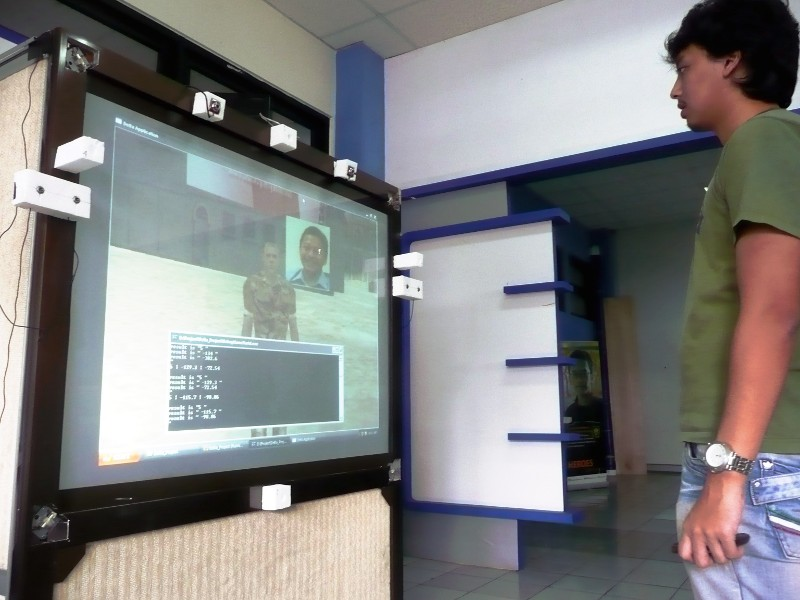
\includegraphics[width=0.9\textwidth,keepaspectratio=true]{images/prototipe_lskk.jpg}
 \caption[Interaksi pengguna dengan prototipe pemandu virtual LSKK yang dibangun dengan RESTU]{Interaksi pengguna dengan prototipe pemandu virtual LSKK yang dibangun dengan RESTU.}
 \label{fig:prototipe_lskk}
\vskip .5em
\end{figure}

Secara umum, RESTU disusun oleh teknologi pemrosesan bahasa alami, pemrosesan suara, pemrosesan citra, grafis 3D, dan kecerdasan artifisial. Teknologi pemrosesan bahasa alami, mencakup teknologi pengenalan suara dan sintesis suara. Teknologi pemrosesan suara digunakan dalam fungsi penentuan lokasi pengguna berdasarkan suara dan teknologi pemrosesan citra digunakan dalam fungsi pengenalan wajah untuk menentukan lokasi pengguna berdasarkan citra. Teknologi grafis digunakan untuk mewujudkan karakter virtual, perilakunya, dan lingkungannya. Sedangkan, teknologi kecerdasan artifisial dimanfaatkan untuk menyusun respons terhadap masukan dari pengguna yang diterima oleh agen berdasarkan pengetahuan yang dimilikinya.

Fungsi-fungsi yang menyusun RESTU tersebut dapat dikelompokkan menjadi dua bagian, yaitu bagian kognitif dan bagian interaksi. Fungsi kecerdasan artifisial menyusun bagian kognitif. Sedangkan, bagian interaksi tersusun dari fungsi pengenalan suara, sintesis suara, penentuan lokasi pengguna baik menggunakan suara mau pun citra, dan antarmuka grafis. Dengan mengikuti pengelompokan tersebut, di sisi implementasi RESTU dibangun dengan menggunakan dua kelompok \textit{server}, yaitu \textit{Artificial Intelligence (AI) Engine Server} dan \textit{User Interface (UI) Engine Server}. UI Engine Server dapat dibagi menjadi \textit{Camera Engine Server}, \textit{Speech Engine Server}, dan \textit{Graphical User Interface (GUI) Engine Server}. Diagram aliran data antar \textit{server}, atau modul yang ada di dalamnya, ditunjukkan oleh \autoref{fig:RESTU_arch}.

\begin{figure}[ht!]
\vskip 1em
\centering
 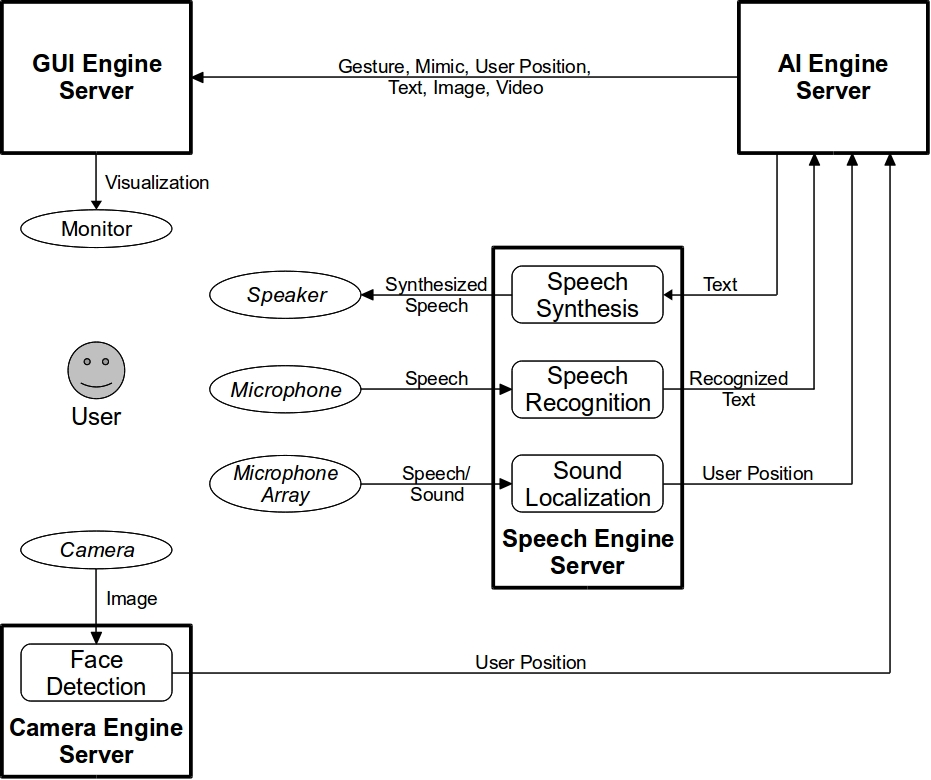
\includegraphics[width=.95\textwidth,keepaspectratio=true]{images/RESTU_arch.jpg}
 \caption[Diagram aliran data RESTU]{Diagram aliran data RESTU.}
 \label{fig:RESTU_arch}
\vskip .5em
\end{figure}


\section{\textit{Speaker Localization} (SpeaCal)}
\label{sec:speacal}

SpeaCal, yang berasal dari istilah \textit{Speaker Localization}, merupakan subsistem penentuan posisi pengguna berdasarkan sinyal suara, yang dalam \autoref{fig:RESTU_arch} disebut sebagai \textit{Sound Localization}. \autoref{sec:speacal} ini akan menguraikan proses perancangan SpeaCal yang menggunakan model perancangan iteratif. Perancangan melalui tahap pendefinisian kebutuhan, penentuan spesifikasi, pembuatan desain, pengimplementasian desain, serta pengujian dan evaluasi. Proses iterasi dilakukan pada tiga tahap yang disebutkan terakhir.

Tahap pembuatan desain meliputi pembuatan desain perangkat lunak dan desain perangkat keras, yang kemudian akan diimplementasikan pada tahap implementasi. Sedangkan, tahap pengujian dan evaluasi meliputi pengambilan data latih dan data uji yang akan digunakan untuk melatih dan menguji JST. Analisis kemudian dilakukan terhadap semua data yang diperoleh, tanpa membedakan antara data latih dan data uji, untuk menentukan apakah desain perangkat lunak dan perangkat keras dapat menghasilkan data yang cukup konsisten sehingga dapat digunakan untuk melatih JST. Apabila data tidak cukup konsisten, proses perancangan akan kembali pada tahap pembuatan desain.

\subsection{Definisi Kebutuhan}

SpeaCal dikembangkan spesifik untuk RESTU. Dari \autoref{chap:pendahuluan} dan \autoref{sec:RESTU}, fungsi penentuan posisi pengguna dibutuhkan untuk mengetahui ke arah mana mata atau kepala agen virtual harus menatap atau menoleh. Dalam komunikasi tatap muka antar manusia, kontak mata diperlukan untuk menunjukkan perhatian terhadap lawan bicara dan topik pembicaraan. meskipun demikian, kontak mata tidak berarti mata seseorang \textit{selalu} menatap lawan bicara \textit{tepat} di matanya selama percakapan.

Dengan demikian, SpeaCal harus dapat menghasilkan informasi \textit{perkiraan} posisi pengguna berdasarkan suara pengguna yang ditangkap oleh mikrofon. Informasi perkiraan posisi yang menjadi prioritas utama adalah informasi \textit{azimuth}. Informasi ini kemudian harus dapat digunakan oleh \textit{AI Engine}, atau \textit{GUI Engine} secara langsung, untuk menentukan ke arah mana mata atau kepala agen virtual harus menatap atau menoleh.

Definisi kebutuhan di atas dapat digambarkan oleh \autoref{fig:speacal_block_diagram}.

\begin{figure}[ht!]
\vskip 1em
\centering
 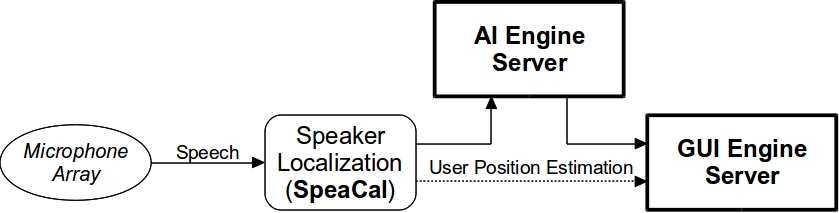
\includegraphics[width=.9\textwidth,keepaspectratio=true]{images/speacal_block_diagram.jpg}
 \caption[Ilustrasi definisi kebutuhan SpeaCal]{Ilustrasi definisi kebutuhan SpeaCal.}
 \label{fig:speacal_block_diagram}
\vskip .5em
\end{figure}

%%%%%%%%%%%%%%%%%%%%%%%%%%%%%%%%%%%%%%%%%%%%%%%%%%5

\subsection{Spesifikasi}
\label{subsec:spesifikasi}

Dari definisi kebutuhan di atas, SpeaCal harus mampu memperkirakan posisi pengguna berdasarkan suara pengguna yang ditangkap oleh mikrofon. Untuk melakukannya, SpeaCal akan menggunakan parameter ITD dan/atau ILD yang membandingkan dua sinyal. Oleh karena itu, diperlukan lebih dari satu mikrofon untuk menangkap suara pengguna. Pada manusia, dua indera pendengaran dapat digunakan untuk memperkirakan \textit{azimuth} posisi sumber suara. Mengacu pada fakta ini, SpeaCal akan menggunakan empat buah mikrofon yang dipasang di bagian atas, bawah, kanan, dan kiri perangkat. Dengan mikrofon-mikrofon tersebut (selanjutnya disebut \textit{microphone array}) diharapkan informasi posisi sumber suara yang diperoleh tidak hanya \textit{azimuth}, tetapi juga \textit{elevation}.

Untuk menangkap sinyal dari mikrofon dibutuhkan \textit{sound card}. Sinyal suara yang akan ditangkap oleh mikrofon adalah suara manusia, sehingga satu kanal suara (mono) saja cukup untuk merepresentasikan sinyal yang ditangkap dengan baik. Dengan demikian, untuk menangkap sinyal dari empat mikrofon dibutuhkan empat kanal suara. Dari hasil survei, \textit{sound card} yang dapat diakses (dibeli) dengan mudah dan harganya murah adalah \textit{USB sound card}. Perangkat seharga Rp 28.000,00 ini memiliki satu kanal masukan yang dapat dimanfaatkan untuk menerima sinyal dari mikrofon.

Untuk mengelola empat \textit{sound card} ini dibutuhkan sebuah program (pustaka) yang mampu mengakses \textit{buffer} yang dimiliki \textit{sound card}, sehingga data sinyal yang tertangkap oleh mikrofon dapat disimpan dalam sebuah file. File-file representasi sinyal dari setiap mikrofon kemudian akan diolah untuk menghitung TDOA, sebagai parameter ITD, dan PtPAR, sebagai parameter ILD. Perhitungan TDOA akan menggunakan DFT agar komputasi dapat dilakukan dengan lebih cepat. Oleh karena itu, dibutuhkan pustaka yang mampu melakukan FFT.

Parameter TDOA dan/atau PtPAR inilah yang kemudian digunakan oleh JST untuk memperkirakan posisi pengguna. Untuk membangun sebuah JST diperlukan kumpulan data latih dan data uji yang memuat nilai masukan, berupa nilai TDOA dan/atau PtPAR, dan nilai keluaran, berupa posisi. Data latih digunakan untuk membangun (melatih) JST, sedangkan data uji digunakan untuk menguji jaringan yang telah dilatih. JST tersebut kemudian digunakan untuk proses penentuan posisi pengguna saat SpeaCal telah diintegrasikan dalam RESTU. Oleh karena itu, dibutuhkan pustaka pustaka yang mampu membangun dan menggunakan JST.

Dengan demikian, SpeaCal harus mampu:

\begin{enumerate}
\item menangkap suara pengguna dengan menggunakan \textit{microphone array}, yang terdiri dari empat mikrofon, secara bersamaan;
\item menghitung TDOA dari sinyal suara yang ditangkap oleh \textit{microphone array};
\item menghitung PtPAR dari sinyal suara yang ditangkap oleh \textit{microphone array};
\item menyimpan data TDOA, PtPAR, dan posisi untuk membuat data latih dan data uji JST;
\item melatih JST dengan nilai TDOA dan PtPAR yang didapatkan selama pengambilan data latih;
\item menguji JST dengan nilai TDOA dan PtPAR yang didapatkan selama pengambilan data uji;
\item menggunakan JST untuk menghasilkan informasi perkiraan posisi pengguna (sumber suara); dan
\item mengirimkan informasi perkiraan posisi pengguna ke subsistem lain (\textit{AI Engine} atau \textit{GUI Engine}).
\end{enumerate}

Perangkat keras yang akan digunakan meliputi:

\begin{itemize}
\item perangkat \textit{multitouch screen} vertikal milik LSKK yang berdimensi 139 x 60 x 180 centimeter (panjang x lebar x tinggi) (\autoref{fig:multitouch-foto}, \autoref{fig:multitouch-dim});

\item komputer:
\begin{itemize}
\item untuk perancangan serta pengambilan data latih dan uji: laptop Dell XPS M1330 dengan prosesor Intel$^{\small{\textregistered}}$~Core\texttrademark~2 Duo T8100 2,1 GHz dan memori 2 GB, dan
\item untuk demo: komputer rakitan dengan prosesor Intel$^{\small{\textregistered}}$~Core\texttrademark~i7 2,67 GHz dan memori 2 GB;
\end{itemize}

\item \textit{USB sound card} tanpa merk (4 buah), dengan dua kanal keluaran yang hanya mendukung \textit{sample rate} 48 KHz dan satu kanal masukan yang hanya mendukung \textit{sample rate} 24 KHz (\autoref{fig:foto_sound_card_dan_hub});

\item \textit{USB hub} merk Belkin, yang memiliki empat \textit{port} (\autoref{fig:foto_sound_card_dan_hub}); 

\item mikrofon (4 buah) merk Genius seri MIC-01A, yang bagian tangkainya dipotong dan bagian kepalanya ditancapkan pada \textit{styrofoam} yang ditempelkan pada perangkat \textit{multitouch screen} vertikal (\autoref{fig:foto_mic_styrofoam}); dan

\item \textit{speaker} merk Genius seri SP-i150;
\end{itemize}

Sedangkan, perangkat lunak yang akan digunakan meliputi:

\begin{itemize}
\item sistem operasi: Ubuntu 10.04.2 LTS;
\item bahasa pemrograman: C, C++;
\item IDE: CodeBlocks;
\item pustaka: C Std Lib, C POSIX Lib, C++ Std Lib, Portaudio, FFTW3, FANN, Boost, wxWidgets;
\item pengolah data: gedit, OpenOffice Calc;
\item pendukung: Audacity, Octave.
\end{itemize}

\begin{figure}[ht!]
\vskip 1em
\centering
 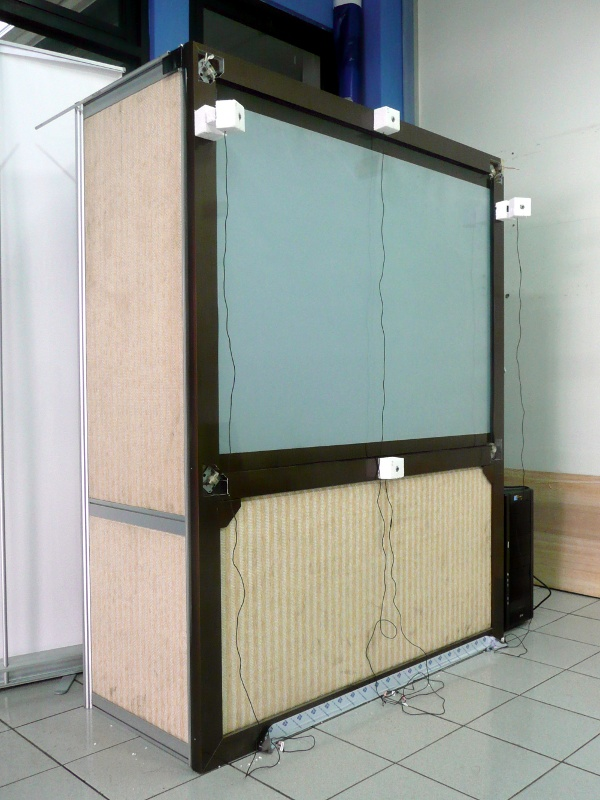
\includegraphics[height=12cm,keepaspectratio=true]{images/multitouch.jpg}
 \caption[Foto perangkat \textit{multitouch screen} vertikal yang akan digunakan untuk demo RESTU]{Foto perangkat \textit{multitouch screen} vertikal yang akan digunakan untuk demo RESTU.}
 \label{fig:multitouch-foto}
\vskip .5em
\end{figure}

\begin{figure}[htp!]
\vskip 1em
\centering
 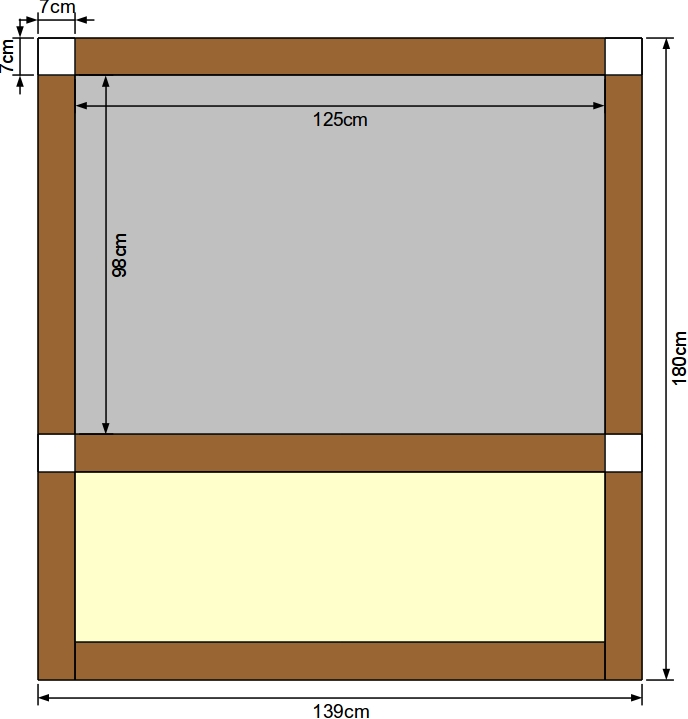
\includegraphics[height=12cm,keepaspectratio=true]{images/multitouch-dim.jpg}
 \caption[Dimensi bagian muka perangkat \textit{multitouch screen} vertikal yang akan digunakan untuk demo RESTU]{Dimensi bagian muka perangkat \textit{multitouch screen} vertikal yang akan digunakan untuk demo RESTU.}
 \label{fig:multitouch-dim}
\vskip .5em
\end{figure}

\begin{figure}[htp!]
\vskip 1em
  \begin{center}
    \subfigure[Foto \textit{USB sound card} dan \textit{USB hub}.]
    {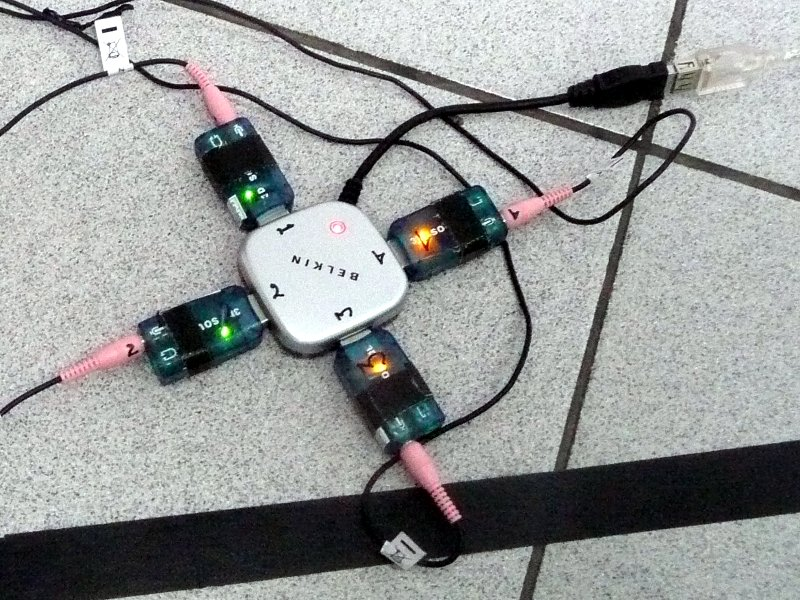
\includegraphics[width=.475\textwidth,keepaspectratio=true]{images/foto_sound_card_dan_hub.jpg}
    \label{fig:foto_sound_card_dan_hub}}
    \subfigure[Foto instalasi mikrofon pada perangkat \textit{multitouch screen} vertikal.]
    {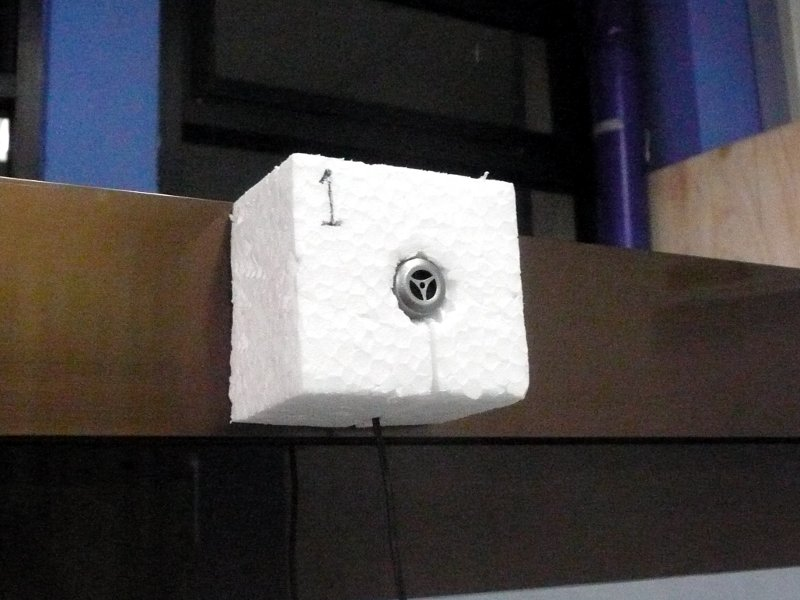
\includegraphics[width=.475\textwidth,keepaspectratio=true]{images/foto_mic_styrofoam.jpg}
    \label{fig:foto_mic_styrofoam}}
  \end{center}
  \caption[Foto \textit{USB sound card}, \textit{USB hub}, dan mikrofon yang digunakan dalam perancangan]{Foto sebagian perangkat keras yang digunakan dalam perancangan.}
  \vskip .5em
\end{figure}


\subsection{Iterasi I: Desain}
\label{subsec:iter1_desain}

\subsubsection{Perangkat Lunak}

Dari \autoref{subsec:spesifikasi} dapat didefinisikan tiga perangkat lunak (program) utama yang dibutuhkan dalam perancangan subsistem penentuan posisi pengguna berdasarkan sinyal suara, yaitu:
\begin{enumerate}
\item SpeaCalTrain, yaitu perangkat lunak (program) yang digunakan untuk memperoleh data latih dan data uji untuk JST;
\item SpeaCal, yaitu perangkat lunak (program) yang digunakan untuk memperkirakan posisi pengguna memanfaatkan JST; dan
\item perangkat lunak (program) pendukung yang digunakan untuk melatih JST dengan memanfaatkan data latih dan mengujinya dengan memanfaatkan data uji.
\end{enumerate}

Dalam \autoref{subsec:spesifikasi} telah dijelaskan bahwa penentuan posisi pengguna akan memanfaatkan parameter TDOA dan PtPAR. Kedua parameter tersebut akan dihitung dari empat sinyal suara yang ditangkap oleh empat mikrofon. Oleh karena itu, fungsi penangkap sinyal suara serta fungsi penghitung parameter TDOA dan PtPAR menjadi inti dari SpeaCalTrain dan SpeaCal. 

\autoref{fig:flowchart_main_wxspeacaltrain} menunjukkan alur program yang digunakan untuk mendapatkan data latih dan data uji untuk JST. \autoref{fig:flowchart_main_wxspeacal} menunjukkan alur program yang digunakan untuk memperkirakan posisi pengguna memanfaatkan JST. Sedangkan, \autoref{fig:flowchart_main_anntraining} menunjukkan alur program yang digunakan untuk melatih JST.

\autoref{fig:flowchart_record_wxspeacaltrain} dan \autoref{fig:flowchart_record_wxspeacal} menunjukkan alur fungsi penangkap sinyal pada SpeaCalTrain dan SpeaCal. Sedangkan, \autoref{fig:flowchart_compute_wxspeacaltrain} dan \autoref{fig:flowchart_compute_wxspeacal} menunjukkan alur fungsi penghitung parameter TDOA dan PtPAR. Pada prinsipnya, fungsi penangkap sinyal suara dan penghitung parameter yang digunakan pada kedua program adalah sama. Perbedaannya terletak pada adanya proses menyimpan data pada program SpeaCalTrain dan adanya proses menjalankan JST pada program SpeaCal.

Durasi sampel sinyal suara yang direkam oleh fungsi penangkap sinyal dapat diatur secara fleksibel. Akan tetapi, perlu diingat bahwa durasi sampel sinyal suara berpengaruh pada banyaknya \textit{frame} yang harus diolah oleh fungsi penghitung parameter. Dari pengamatan, durasi sampel berbanding lurus dengan waktu yang dibutuhkan oleh fungsi penghitung parameter untuk menyelesaikan operasinya. Oleh karena itu, apabila durasi sampel sinyal diset $x$ detik, fungsi penangkap sinyal harus diset ke \textit{idle} selama $x$ detik setiap kali selesai merekam sinyal selama $x$ detik untuk memastikan bahwa fungsi penghitung parameter telah menyelesaikan operasinya. Dalam perancangan ini, durasi yang digunakan adalah 0,5 dan 1 detik, sehingga nilai perkiraan posisi pengguna diperbarui setiap 1 dan 2 detik.

Data yang disimpan pada program SpeaCalTrain terdiri dari data suara dalam file berekstensi \texttt{raw} dan data TDOA serta PtPAR yang tertulis dalam sebuah file teks. Format penulisan file teks yang memuat data TDOA dan PtPAR disesuaikan dengan format data latih JST. Contoh penulisan file teks data tersebut dapat dilihat pada \autoref{lst:teks_data}. Baris pertama dalam file menunjukkan jumlah data (pasangan masukan dan keluaran) yang tercantum dalam file tersebut, jumlah masukan, dan jumlah keluaran. Dalam contoh yang tercantum pada \autoref{lst:teks_data}, jumlah data adalah 120, jumlah masukan 12, dan jumlah keluaran 3. Baris-baris selanjutnya terbagi atas dua macam, yaitu baris genap menuliskan data masukan dan baris ganjil menuliskan data keluaran yang bersesuaian. Dalam contoh yang tercantum pada \autoref{lst:teks_data}, baris data masukan mencantumkan enam data TDOA yang disusul dengan enam data PtPAR dan baris data keluaran mencantumkan representasi sebuah titik dalam koordinat Cartesian.

\singlespacing
\begin{figure}[htp!]
\vskip 1em
\begin{lstlisting}
120	12	3
1.375	2.833	3.208	1.417	1.792	0.417	-7.214	-11.371	-15.296	-4.156	-8.081	-3.925
190	30	60
-1.458	2.500	1.292	3.833	2.667	-1.125	-7.244	-11.366	-15.586	-4.121	-8.341	-4.220
190	30	60
0.000	7.292	2.667	2.917	2.667	-0.250	-7.097	-11.227	-15.222	-4.130	-8.125	-3.995
190	30	60
...
\end{lstlisting}
\caption[Contoh penulisan data TDOA dan PtPAR dalam file teks data]{Contoh penulisan data TDOA dan PtPAR dalam file teks data.}
\label{lst:teks_data}
\vskip .5em
\end{figure}
\onehalfspacing

\begin{figure}[htp!]
\vskip 1em
\centering
 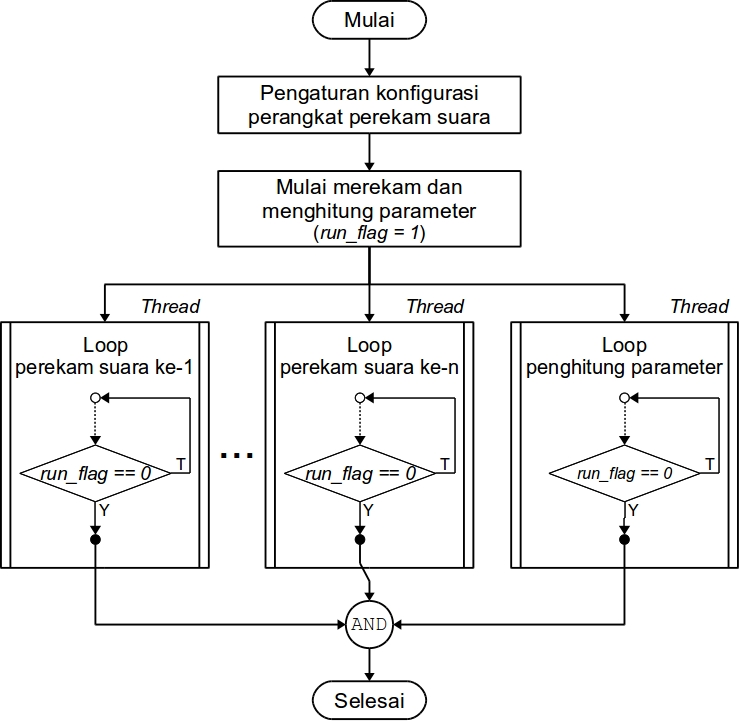
\includegraphics[scale=.5,keepaspectratio=true]{images/flowchart_main_wxspeacaltrain.jpg}
 \caption[Diagram alir SpeaCalTrain]{Diagram alir SpeaCalTrain.}
 \label{fig:flowchart_main_wxspeacaltrain}
\vskip .5em
\end{figure}

\begin{figure}[htp!]
\vskip 1em
\centering
 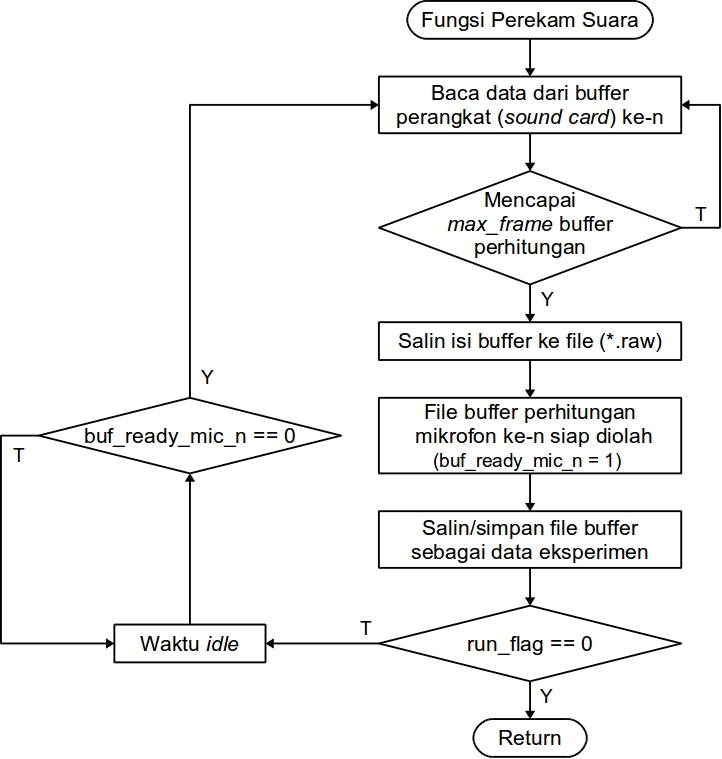
\includegraphics[scale=.5,keepaspectratio=true]{images/flowchart_record_wxspeacaltrain.jpg}
 \caption[Diagram alir fungsi perekam suara pada SpeaCalTrain]{Diagram alir fungsi perekam suara pada SpeaCalTrain.}
 \label{fig:flowchart_record_wxspeacaltrain}
\vskip .5em
\end{figure}

\begin{figure}[htp!]
\vskip 1em
\centering
 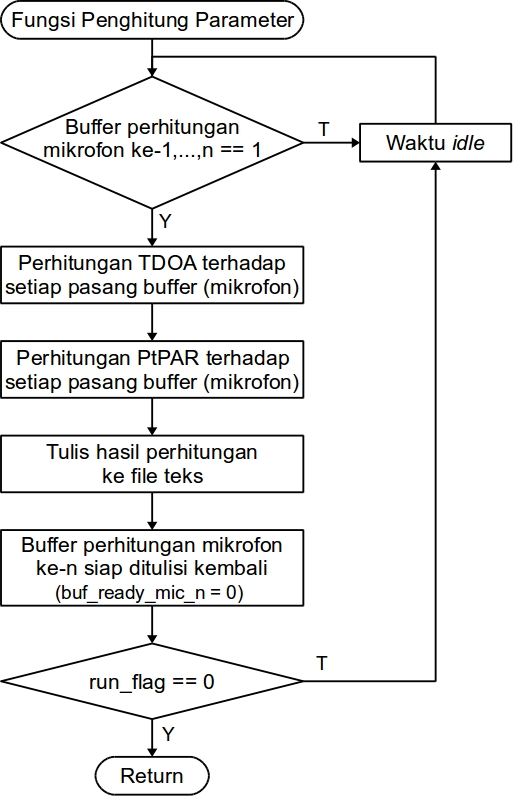
\includegraphics[scale=.5,keepaspectratio=true]{images/flowchart_compute_wxspeacaltrain.jpg}
 \caption[Diagram alir fungsi penghitung parameter TDOA dan PtPAR pada SpeaCalTrain]{Diagram alir fungsi penghitung parameter TDOA dan PtPAR pada SpeaCalTrain.}
 \label{fig:flowchart_compute_wxspeacaltrain}
\vskip .5em
\end{figure}

\begin{figure}[htp!]
\vskip 1em
\centering
 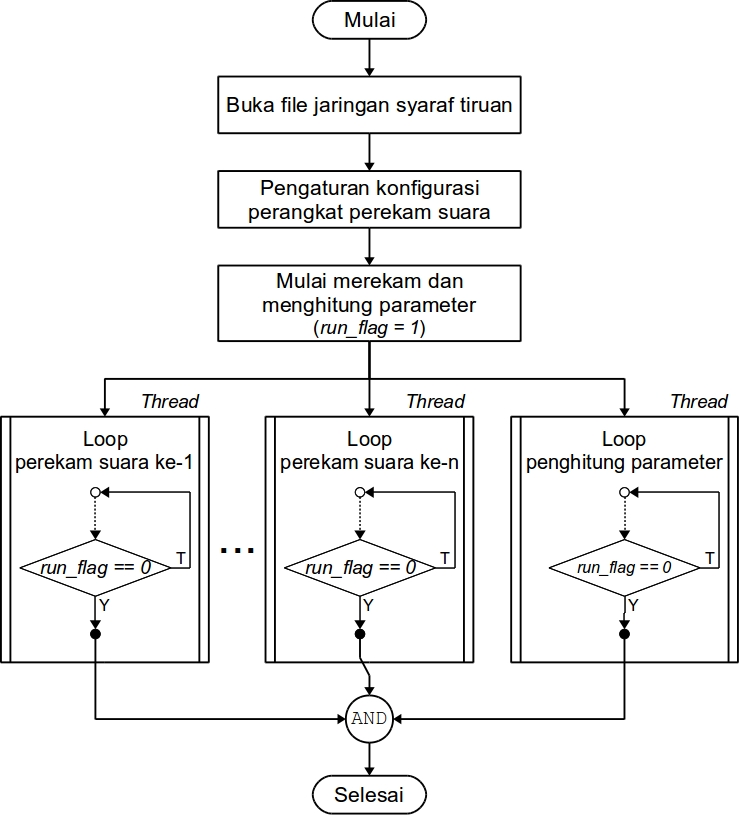
\includegraphics[scale=.5,keepaspectratio=true]{images/flowchart_main_wxspeacal.jpg}
 \caption[Diagram alir SpeaCal]{Diagram alir SpeaCal.}
 \label{fig:flowchart_main_wxspeacal}
\vskip .5em
\end{figure}

\begin{figure}[htp!]
\vskip 1em
\centering
 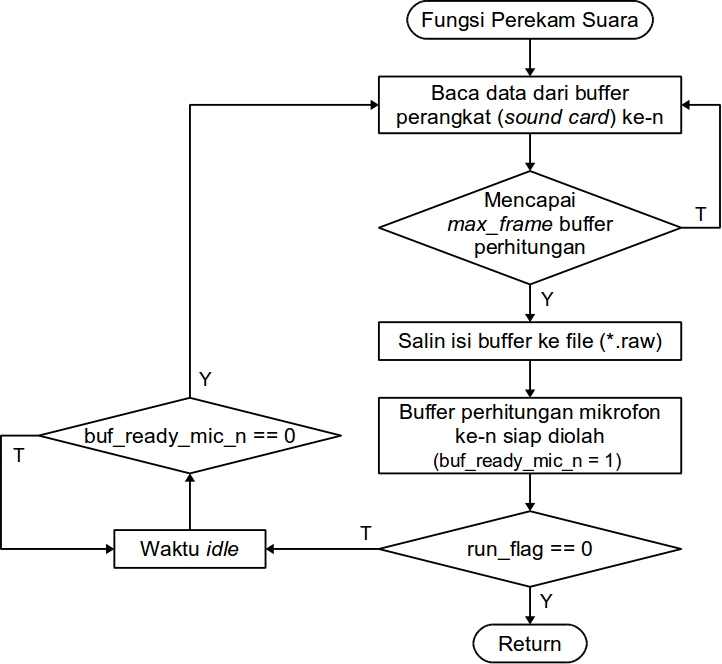
\includegraphics[scale=.5,keepaspectratio=true]{images/flowchart_record_wxspeacal.jpg}
 \caption[Diagram alir fungsi perekam suara pada SpeaCal]{Diagram alir fungsi perekam suara pada SpeaCal.}
 \label{fig:flowchart_record_wxspeacal}
\vskip .5em
\end{figure}

\begin{figure}[htp!]
\vskip 1em
\centering
 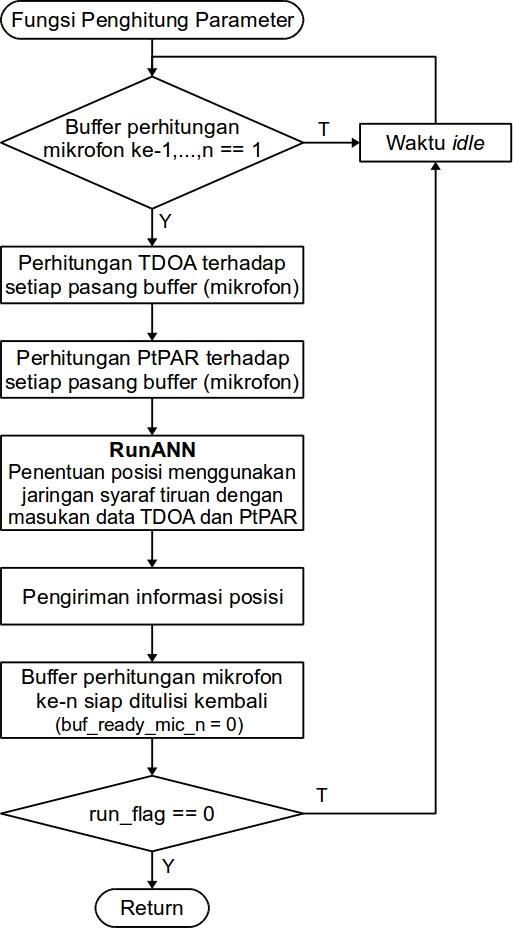
\includegraphics[scale=.5,keepaspectratio=true]{images/flowchart_compute_wxspeacal.jpg}
 \caption[Diagram alir fungsi penghitung parameter TDOA dan PtPAR pada SpeaCal]{Diagram alir fungsi penghitung parameter TDOA dan PtPAR pada SpeaCal.}
 \label{fig:flowchart_compute_wxspeacal}
\vskip .5em
\end{figure}

\begin{figure}[ht!]
\vskip 1em
\centering
 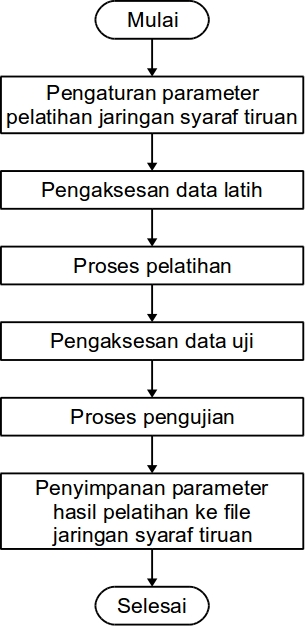
\includegraphics[scale=.5,keepaspectratio=true]{images/flowchart_main_anntraining.jpg}
 \caption[Diagram alir program untuk melatih JST]{Diagram alir program untuk melatih JST.}
 \label{fig:flowchart_main_anntraining}
\vskip .5em
\end{figure}


\subsubsection{Perangkat Keras}

Dalam penentuan posisi pengguna berdasarkan TDOA dan PtPAR, penempatan mikrofon akan sangat berpengaruh. Empat mikrofon yang digunakan akan ditempatkan pada perangkat \textit{multitouch} vertikal seperti yang ditunjukkan oleh \autoref{fig:desain_mic_1}. Dengan desain tersebut diharapkan posisi pengguna dalam ruang dapat diperkirakan. Apabila manusia dapat memperkirakan \textit{azimuth} posisi sumber suara dengan dua telinga, secara logis \textit{azimuth} posisi pengguna dapat diperkirakan dengan membandingkan sinyal yang tertangkap oleh mikrofon kanan dan kiri, sedangkan \textit{elevation} dapat diperkirakan dengan sinyal dari mikrofon atas dan bawah. Selain itu, dengan adanya perbedaan jarak mikrofon kanan-kiri dan mikrofon atas-bawah terhadap permukaan layar, diharapkan jarak pengguna terhadap layar juga dapat diperkirakan memanfaatkan parameter TDOA dan PtPAR yang membandingkan kombinasi mikrofon kanan-kiri dan mikrofon atas-bawah, misalnya parameter TDOA dan PtPAR pasangan mikrofon atas dan kanan. meskipun demikian, prioritas utama adalah memperolah \textit{azimuth} posisi pengguna relatif terhadap perangkat \textit{multitouch}.

\addtocontents{lof}{\vspace{4em} \hfill {Halaman} \par}

\begin{figure}[ht!]
\vskip 1em
  \begin{center}
    \subfigure[Tampak muka]
    {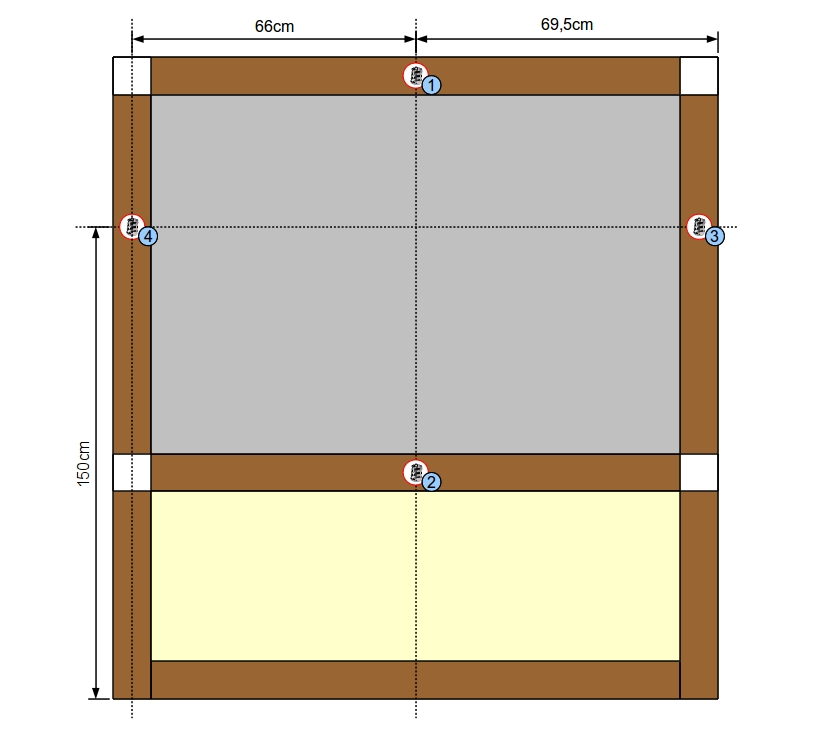
\includegraphics[scale=.5,keepaspectratio=true]{images/desain_mic_1a.jpg}
    \label{fig:desain_mic_1a}}
    \subfigure[Tampak atas]
    {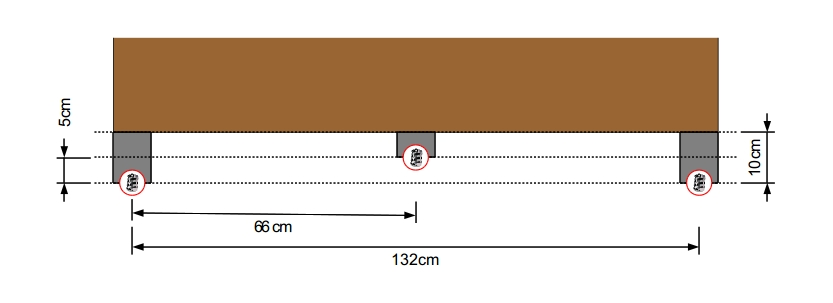
\includegraphics[scale=.5,keepaspectratio=true]{images/desain_mic_1b.jpg}
    \label{fig:desain_mic_1b}}
  \end{center}
  \caption[Rancangan penempatan mikrofon]{Rancangan penempatan mikrofon.}
  \label{fig:desain_mic_1}
  \vskip .5em
\end{figure}


\subsubsection{Pengambilan Data}

Pengambilan data latih dan uji untuk JST dilakukan dengan menempatkan sumber suara (\textit{speaker}) pada koordinat tertentu relatif terhadap perangkat \textit{multitouch} vertikal. Titik 0 dari koordinat Cartesian yang digunakan adalah ujung kiri atas perangkat \textit{multitouch}. Pengguna diasumsikan merupakan manusia dewasa dengan tinggi 160-170 cm. Dengan demikian, dapat diasumsikan bahwa posisi mulut berada pada ketinggian 150 cm dari tanah. Oleh karena itu, sumber suara ditempatkan pada koordinat $z = -30$, sedangkan koordinat $x$ dan $y$ merupakan variabel. Jangkauan nilai kedua koordinat tersebut adalah $x = \{-50, 10, 70, 130, 190\}$ dan $y = \{60, 120, 180\}$ (ditandai dengan tanda X pada \autoref{fig:floor_plan_1}).

\begin{figure}[ht!]
\vskip 1em
\centering
 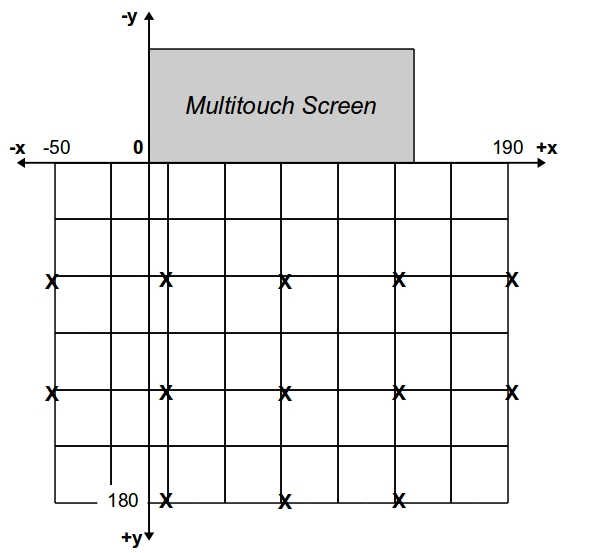
\includegraphics[scale=.5,keepaspectratio=true]{images/floor_plan_1.jpg}
 \caption[Rancangan titik pengambilan data]{Rancangan titik pengambilan data.}
 \label{fig:floor_plan_1}
\vskip .5em
\end{figure}


\subsection{Iterasi I: Implementasi}

\subsubsection{Perangkat Lunak}

Implementasi fungsi perekam suara memanfaatkan pustaka Portaudio untuk mengakses \textit{buffer} yang dimiliki \textit{sound card} dan menyalinnya ke sebuah file yang berekstensi \texttt{raw}. File-file yang berisi representasi sinyal suara dari empat mikrofon inilah yang kemudian akan diolah oleh fungsi penghitung parameter.

\singlespacing
\begin{figure}[htp!]
\vskip 1em
\begin{lstlisting}
if(inputBuffer == NULL)
{
	for(i=0; i<framesPerBuffer; i++)
    {
		output_data_buffer[i] = SAMPLE_SILENCE;  /* left */
		if(NUM_CHANNELS == 2)
			output_data_buffer[i] = SAMPLE_SILENCE;  /* right */
	}
}
else
{
	for(i=0; i<framesPerBuffer; i++)
	{
		output_data_buffer[i] = *input++;
	}
}
\end{lstlisting}
\caption[Kode program operasi pembacaan data dari \textit{buffer} yang dimiliki \textit{sound card}]{Kode program operasi pembacaan data dari \textit{buffer} yang dimiliki \textit{sound card}.}
\label{lst:read_sound_card_buffer}
\vskip .5em
\end{figure}
\onehalfspacing

\singlespacing
\begin{figure}[htp!]
\vskip 1em
\begin{lstlisting}
sprintf(recordFileName,"dev-%d-buf-rec-%d.raw", userDataFile->devNum, pubBufFileID);
buf_fid = fopen(recordFileName, "wb");
if(buf_fid == NULL)
{
	printf("Could not open file for saving the buffer.");
	exit(1);
}
else
{
	fwrite(output_data_buffer, NUM_CHANNELS * sizeof(SAMPLE), framesPerBuffer, buf_fid);
	fclose(buf_fid);
}
\end{lstlisting}
\caption[Kode program operasi penyimpanan data ke file yang berekstensi \texttt{raw}]{Kode program operasi penyimpanan data ke file yang berekstensi \texttt{raw}.}
\label{lst:save_data_to_raw_file}
\vskip .5em
\end{figure}
\onehalfspacing


Fungsi penghitung parameter terdiri dari penghitung parameter TDOA dan PtPAR. Metode CCC digunakan untuk menghitung TDOA dari sepasang data sinyal. Untuk memperoleh operasi yang cepat, metode CCC diimplentasikan menggunakan DFT. Oleh karena itu, fungsi ini memanfaatkan pustaka FFTW3 dalam proses penghitungan TDOA. \autoref{lst:ccc_op} menunjukkan implementasi metode CCC. Parameter TDOA dapat diperoleh dengan mencari nilai maksimum dari hasil operasi CCC.

\singlespacing
\begin{figure}[htp!]
\vskip 1em
\begin{lstlisting}
pa = fftw_plan_dft_1d((N << 1) - 1, signala_ext, outa, FFTW_FORWARD, FFTW_ESTIMATE);
pb = fftw_plan_dft_1d((N << 1) - 1, signalb_ext, outb, FFTW_FORWARD, FFTW_ESTIMATE);
px = fftw_plan_dft_1d((N << 1) - 1, out, out_shifted, FFTW_BACKWARD, FFTW_ESTIMATE);

for (i = 0; i < (N << 1) - 1; i++) {
	if (i < N) {
		signala_ext[i] = signala[i];
		signalb_ext[i] = signalb[i];
	}
	else {
		signala_ext[i] = 0;
		signalb_ext[i] = 0;
	}
}

fftw_execute(pa);
fftw_execute(pb);

for (i = 0; i < (N << 1) - 1; i++)
	out[i] = outa[i] * conj(outb[i]);

fftw_execute(px);

for (i = 0; i < (N << 1) - 1; i++)
	result[i] = out_shifted[(i + N) % ((N << 1) - 1)] / ((N << 1) - 1);
\end{lstlisting}
\caption[Kode program operasi CCC terhadap dua data sinyal]{Kode program operasi CCC terhadap dua data sinyal.}
\label{lst:ccc_op}
\vskip .5em
\end{figure}
\onehalfspacing


\singlespacing
\begin{figure}[htp!]
\vskip 1em
\begin{lstlisting}
maxTemp1 = minTemp1 = creal(first_xcorr_signal[0]);;
maxTemp2 = minTemp2 = creal(second_xcorr_signal[0]);

for(l = 0; l < FramesPerBuffer; l++) {
	if(creal(first_xcorr_signal[l]) > maxTemp1)
		maxTemp1 = creal(first_xcorr_signal[l]);
	if(creal(first_xcorr_signal[l]) < minTemp1)
		minTemp1 = creal(first_xcorr_signal[l]);
	if(creal(second_xcorr_signal[l]) > maxTemp2)
		maxTemp2 = creal(second_xcorr_signal[l]);
	if(creal(second_xcorr_signal[l]) < minTemp2)
		minTemp2 = creal(second_xcorr_signal[l]);
}

return 20*log10((maxTemp1-minTemp1)/(maxTemp2-minTemp2));
\end{lstlisting}
\caption[Kode program operasi perhitungan PtPAR]{Kode program operasi perhitungan PtPAR.}
\label{lst:ptpar_op}
\vskip .5em
\end{figure}
\onehalfspacing


\subsubsection{Perangkat Keras}

Implementasi rancangan penempatan mikrofon dapat dilihat pada \autoref{fig:desain_mic_1c}. Mikrofon ditancapkan pada \textit{styrofoam} yang ditempelkan pada perangkat \textit{multitouch} vertikal (\autoref{fig:desain_mic_2c2}). Selain sebagai tempat untuk meletakkan mikrofon, \textit{styrofoam} juga dapat berfungsi sebagai peredam suara. Oleh karena itu, diharapkan mikrofon hanya menangkap sinyal suara dari arah depan.

\begin{figure}[ht!]
\vskip 1em
\centering
 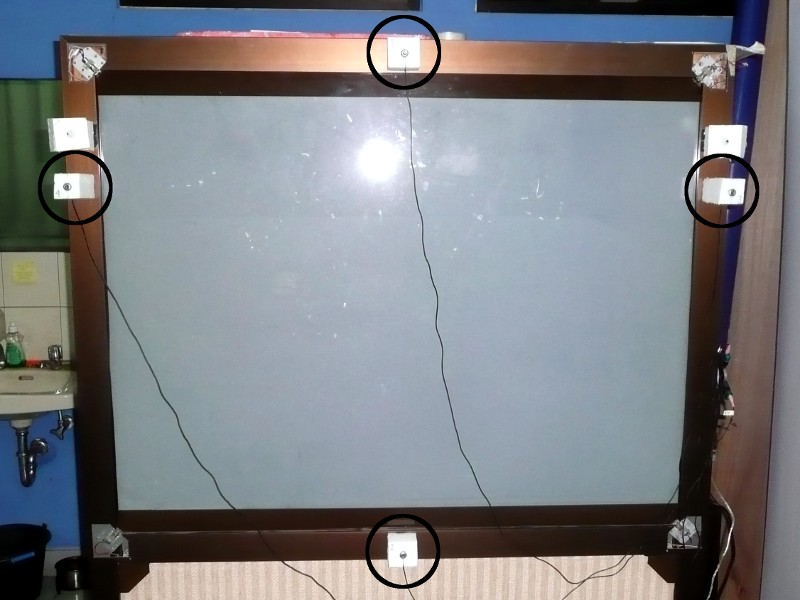
\includegraphics[width=.9\textwidth,keepaspectratio=true]{images/desain_mic_1c.jpg}
 \caption[Foto implementasi rancangan penempatan mikrofon]{Foto implementasi rancangan penempatan mikrofon.}
 \label{fig:desain_mic_1c}
\vskip .5em
\end{figure}


\subsection{Iterasi I: Pengujian dan Evaluasi}

Pengambilan data dilakukan dengan memutar secara berulang-ulang file rekaman suara FAN\_1A dan MAA\_1A yang berisi ucapan kata "satu". Masing-masing rekaman menghasilkan sebuah set data yang memuat 78 data dari 13 titik pengambilan data yang telah didefinisikan pada \autoref{subsec:iter1_desain} (6 data per titik). \autoref{fig:1_fan_1a_34}  dan \autoref{fig:1_maa_1a_34} menunjukkan parameter TDOA dan PtPAR pasangan mikrofon 3 dan 4 dari set data FAN\_1A dan MAA\_1A. Untuk memudahkan pembacaan grafik, jangkauan nilai koordinat $x = \{-50, 10, 70, 130, 190\}$ dan $y = \{60, 120, 180\}$ diubah menjadi $x = \{-2, -1, 0, 1, 2\}$ dan $y = \{-1, 0, 1\}$.

Grafik-grafik dari dua set data tersebut memperlihatkan bahwa nilai parameter PtPAR tidak cukup konsisten dan nilai parameter TDOA sangat tidak konsisten. Dua set data ini tidak dapat digunakan untuk  melatih JST yang baik.

\begin{figure}[htp!]
\vskip 1em
  \begin{center}
    \subfigure[PtPAR]
    {\fbox{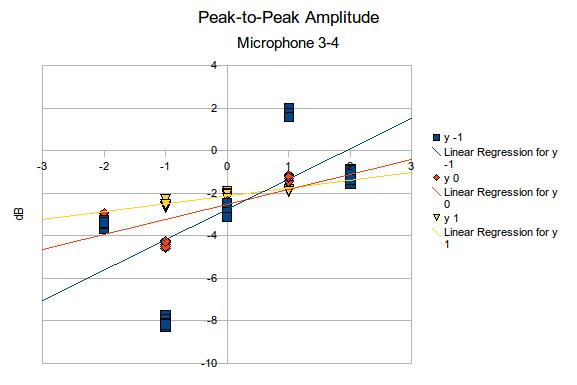
\includegraphics[scale=.55,keepaspectratio=true]{images/1_ptpar_fan_1a_34.jpg}
    \label{fig:1_ptpar_fan_1a_34}}}
    \subfigure[TDOA]
    {\fbox{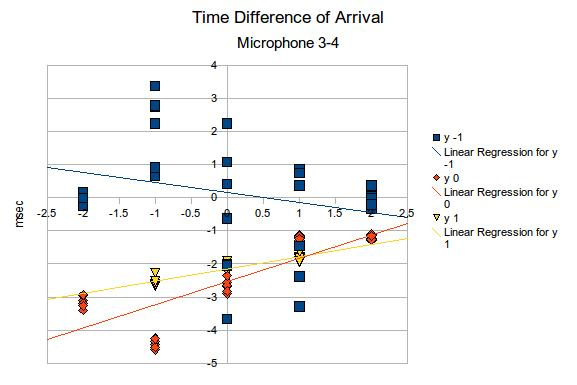
\includegraphics[scale=.55,keepaspectratio=true]{images/1_tdoa_fan_1a_34.jpg}
    \label{fig:1_tdoa_fan_1a_34}}}
  \end{center}
  \caption[Grafik TDOA dan PtPAR mikrofon 3-4 dari set data FAN\_1A]{Grafik TDOA dan PtPAR mikrofon 3-4 dari set data FAN\_1A.}
  \label{fig:1_fan_1a_34}
  \vskip .5em
\end{figure}

\begin{figure}[htp!]
\vskip 1em
  \begin{center}
    \subfigure[PtPAR]
    {\fbox{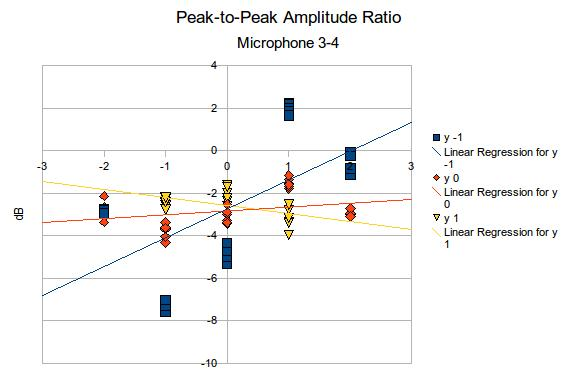
\includegraphics[scale=.55,keepaspectratio=true]{images/1_ptpar_maa_1a_34.jpg}
    \label{fig:1_ptpar_maa_1a_34}}}
    \subfigure[TDOA]
    {\fbox{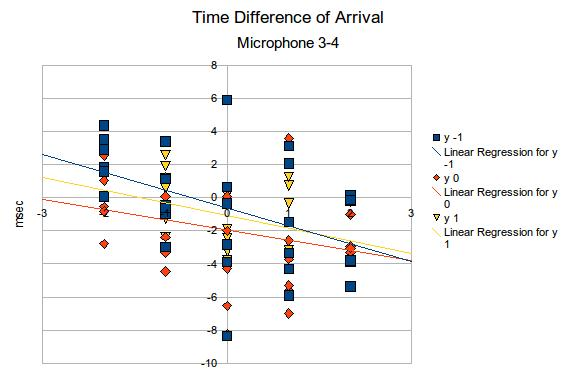
\includegraphics[scale=.55,keepaspectratio=true]{images/1_tdoa_maa_1a_34.jpg}
    \label{fig:1_tdoa_maa_1a_34}}}
  \end{center}
  \caption[Grafik TDOA dan PtPAR mikrofon 3-4 dari set data MAA\_1A]{Grafik TDOA dan PtPAR mikrofon 3-4 dari set data MAA\_1A.}
  \label{fig:1_maa_1a_34}
  \vskip .5em
\end{figure}

\subsection{Iterasi II: Desain}
\label{subsec:iter2_desain}

\subsubsection{Perangkat Keras}

Oleh karena prioritas utama adalah menentukan \textit{azimuth} posisi pengguna relatif terhadap layar, penempatan mikrofon diubah menjadi seperti yang terlihat pada \autoref{fig:desain_mic_2}. Dengan perubahan desain ini, pendekatan terhadap masalah TDOA berubah dari seperti yang tergambar pada \autoref{fig:tdoa_before} menjadi seperti yang tergambar pada \autoref{fig:tdoa_after1} dan \autoref{fig:tdoa_after2}. Selain itu, lebih banyak pasangan mikrofon yang dapat digunakan untuk memperkirakan \textit{azimuth} posisi pengguna relatif terhadap layar. Dengan demikian, terdapat enam parameter yang berpotensi sebagai masukan JST, yaitu dua nilai TDOA dari dua pasang mikrofon yang saling berdekatan dan empat nilai PtPAR dari empat pasang mikrofon yang saling berjauhan. Dua nilai PtPAR dari dua pasang mikrofon yang saling berdekatan dapat diabaikan karena perbedaan amplitudo sinyal yang tertangkap oleh sepasang mikrofon yang letaknya berdekatan tidak signifikan.

\begin{figure}[htp!]
\vskip 1em
  \begin{center}
    \subfigure[Tampak muka]
    {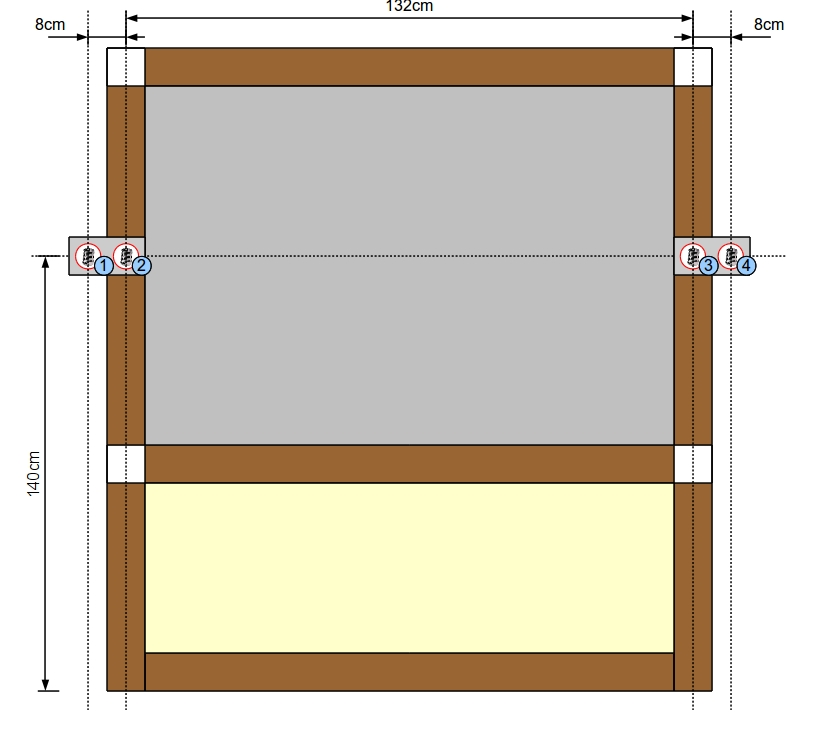
\includegraphics[scale=.5,keepaspectratio=true]{images/desain_mic_2a.jpg}
    \label{fig:desain_mic_2a}}
    \subfigure[Tampak atas]
    {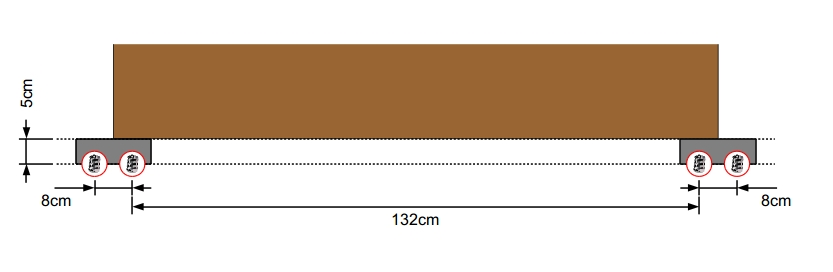
\includegraphics[scale=.5,keepaspectratio=true]{images/desain_mic_2b.jpg}
    \label{fig:desain_mic_2b}}
  \end{center}
  \caption[Perbaikan rancangan penempatan mikrofon]{Perbaikan rancangan penempatan mikrofon.}
  \label{fig:desain_mic_2}
  \vskip .5em
\end{figure}

\begin{figure}[htp!]
\vskip 1em
  \begin{center}
    \subfigure[]
    {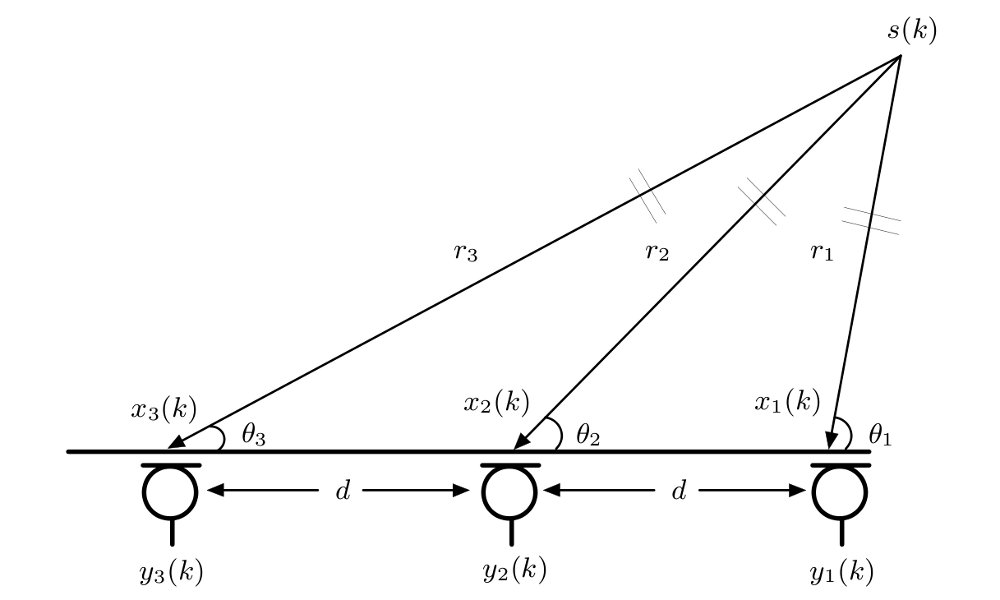
\includegraphics[scale=1.2,keepaspectratio=true]{images/tdoa_before.jpg}
    \label{fig:tdoa_before}}
    \subfigure[]
    {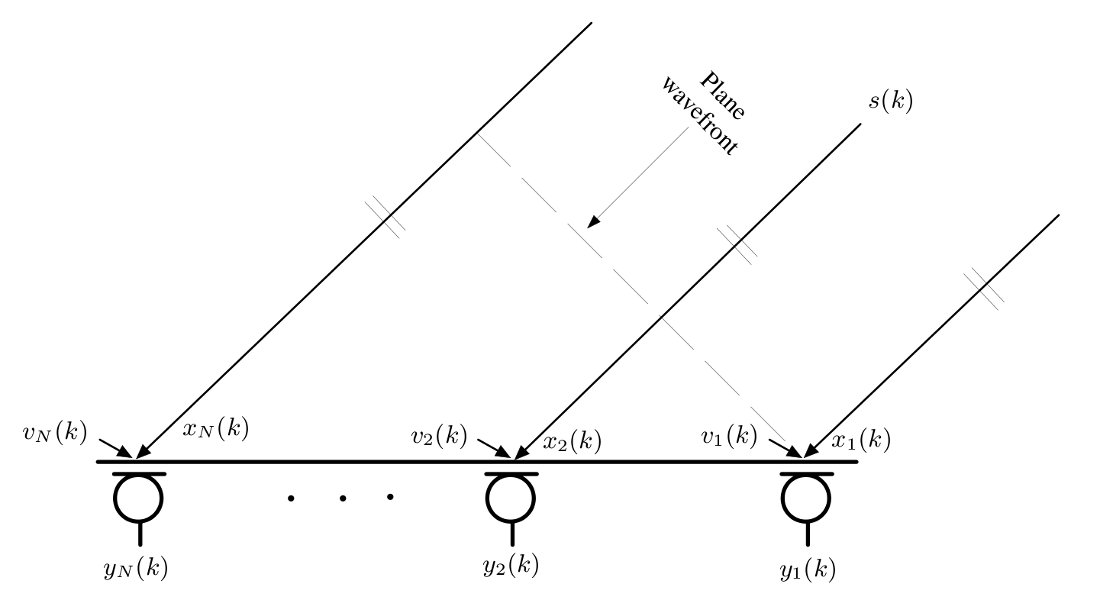
\includegraphics[scale=1.2,keepaspectratio=true]{images/tdoa_after1.jpg}
    \label{fig:tdoa_after1}}
    \subfigure[]
    {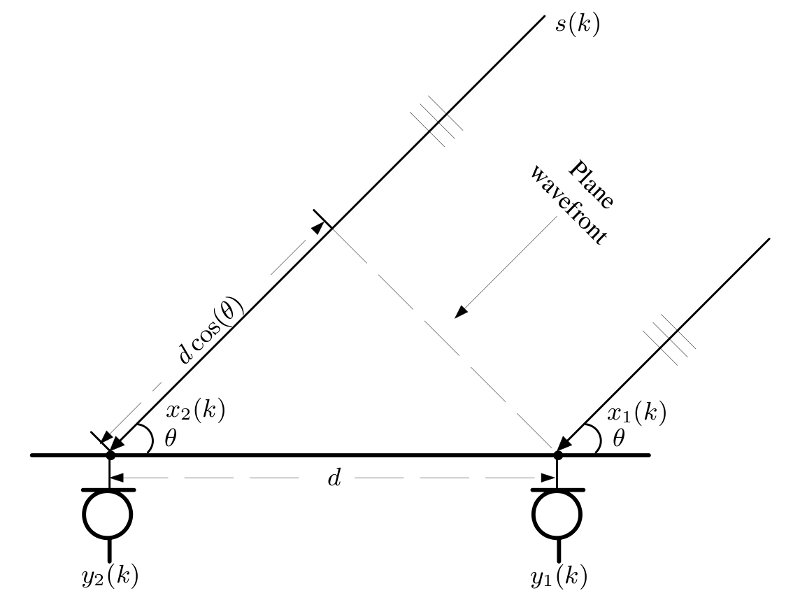
\includegraphics[scale=1.2,keepaspectratio=true]{images/tdoa_after2.jpg}
    \label{fig:tdoa_after2}}
  \end{center}
  \caption[Ilustrasi perubahan pendekatan masalah TDOA]{Ilustrasi perubahan pendekatan masalah TDOA \cite{benesty2008}.}
  \label{fig:tdoa_change}
  \vskip .5em
\end{figure}


\subsubsection{Pengambilan Data}

Jangkauan nilai koordinat sumber suara sama dengan yang digunakan sebelumnya (Iterasi I), yaitu $x = \{-50, 10, 70, 130, 190\}$, $y = \{60, 120, 180\}$, dan $z = -30$. Akan tetapi, titik-titik pengambilan data tersebut kemudian dibagi dalam kawasan-kawasan seperti yang ditunjukkan oleh \autoref{fig:floor_plan_2}. Oleh karena itu, apabila sebelumnya kemungkinan keluaran penentuan posisi pengguna adalah sebuah titik dalam koordinat Cartesian tiga dimensi yang relatif terhadap perangkat \textit{multitouch}, dengan penggunaan kawasan kemungkinan keluaran adalah sebuah sudut (\textit{azimuth}) yang relatif terhadap titik tengah perangkat \textit{multitouch}.

\begin{figure}[ht!]
\vskip 1em
\centering
 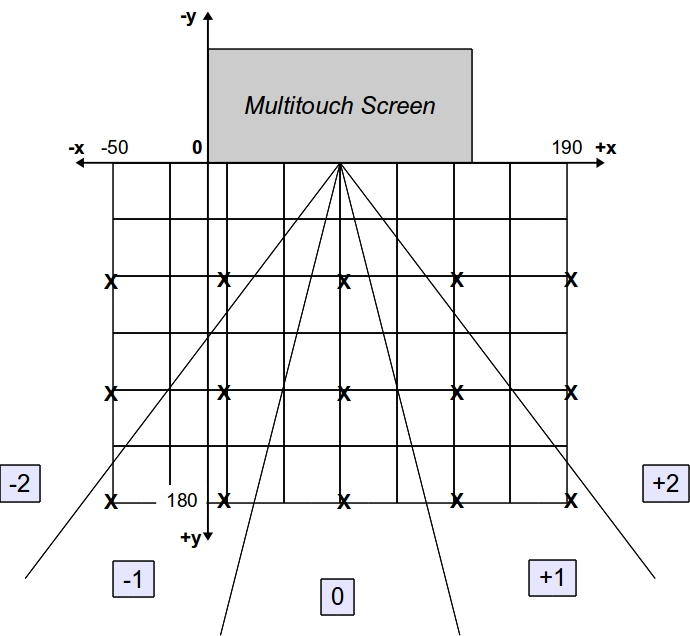
\includegraphics[scale=.5,keepaspectratio=true]{images/floor_plan_2.jpg}
 \caption[Perbaikan rancangan titik pengambilan data]{Perbaikan rancangan titik pengambilan data.}
 \label{fig:floor_plan_2}
\vskip .5em
\end{figure}

%%%%%%%%%%%%%%%%%%%%%%%%%%%%%%%%%%%%%%%%%%%%%%%%%%%%%%%%%%%%%%

\subsection{Iterasi II: Implementasi}

\subsubsection{Perangkat Keras}

Implementasi perbaikan rancangan penempatan mikrofon dapat dilihat pada \autoref{fig:desain_mic_2c1}. \autoref{fig:desain_mic_2c2} menunjukkan bagaimana mikrofon diletakkan dalam \textit{styrofoam} yang ditempelkan pada perangkat \textit{multitouch}.


\begin{figure}[ht!]
\vskip 1em
  \begin{center}
    \subfigure[]
    {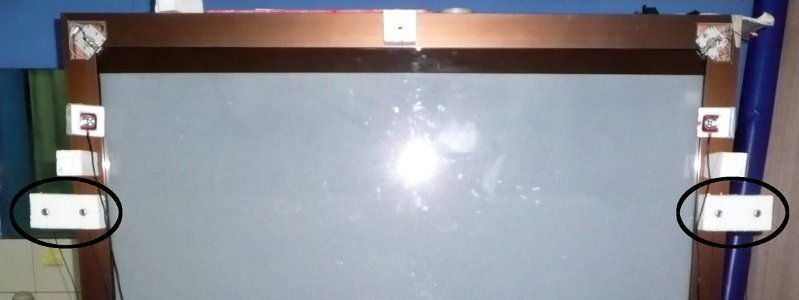
\includegraphics[width=.9\textwidth,keepaspectratio=true]{images/desain_mic_2c1.jpg}
    \label{fig:desain_mic_2c1}}
    \subfigure[]
    {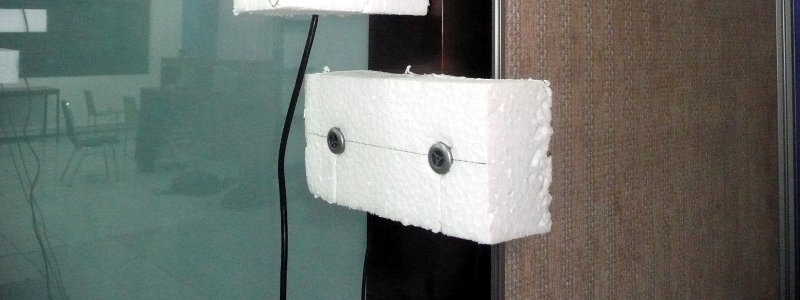
\includegraphics[width=.9\textwidth,keepaspectratio=true]{images/desain_mic_2c2.jpg}
    \label{fig:desain_mic_2c2}}
  \end{center}
  \caption[Foto implementasi perbaikan rancangan penempatan mikrofon]{Foto implementasi perbaikan rancangan penempatan mikrofon.}
  \label{fig:desain_mic_2c}
  \vskip .5em
\end{figure}

%%%%%%%%%%%%%%%%%%%%%%%%%%%%%%%%%%%%%%%%%%%%%%%%%%%%%%%%%%%%%%

\subsection{Iterasi II: Pengujian dan Evaluasi}

Dalam tahap ini, pengambilan data menggunakan empat file rekaman suara, yaitu FAN\_9B (ucapan kata "sembilan"), FAW\_7B (ucapan kata "tujuh"), MAF\_25A (ucapan frase "dua lima"), dan MSD\_5B (ucapan kata "lima"). Untuk memudahkan pembacaan grafik, jangkauan nilai koordinat $x = \{-50, 10, 70, 130, 190\}$ dan $y = \{60, 120, 180\}$ diubah menjadi $x = \{-4, -2, 0, 2, 4\}$ dan $y = \{-2, -4, -6\}$. 

Dari pengamatan terhadap empat set data, nilai parameter PtPAR cukup konsisten, sedangkan nilai parameter TDOA masih saja tidak konsisten. Dengan data tersebut, penentuan posisi pengguna diputuskan hanya akan menggunakan parameter PtPAR saja. Secara lebih spesifik, parameter PtPAR yang akan digunakan adalah parameter PtPAR mikrofon 1-3, 1-4, 2-3, dan 2-4.

Grafik TDOA dan PtPAR yang akan ditampilkan secara lengkap hanya set data FAN\_9B yang cukup merepresentasikan set data yang lain (\autoref{fig:2_fan_9b_tdoa_1} sampai dengan \autoref{fig:2_fan_9b_ptpar_3}). \autoref{fig:2_faw_7b_ptpar_1} dan \autoref{fig:2_faw_7b_ptpar_2} menunjukkan grafik PtPAR mikrofon 1-3, 1-4, 2-3, dan 2-4 dari set data FAW\_7B untuk memberikan gambaran lebih lanjut mengenai data latih dan data uji JST.

\begin{figure}[htp!]
\vskip 1em
  \begin{center}
    \subfigure[TDOA 1-2]
    {\fbox{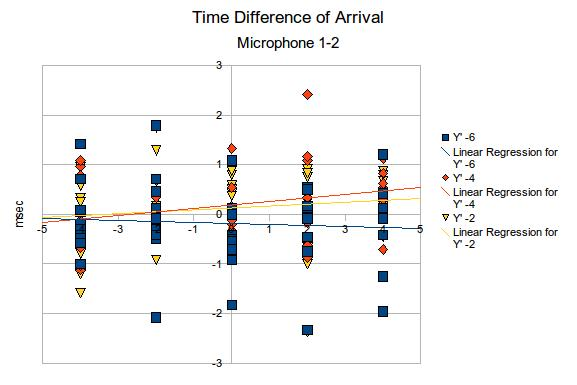
\includegraphics[scale=.55,keepaspectratio=true]{images/2_fan_9b_tdoa_12.jpg}
    \label{fig:2_fan_9b_tdoa_12}}}
    \subfigure[TDOA 3-4]
    {\fbox{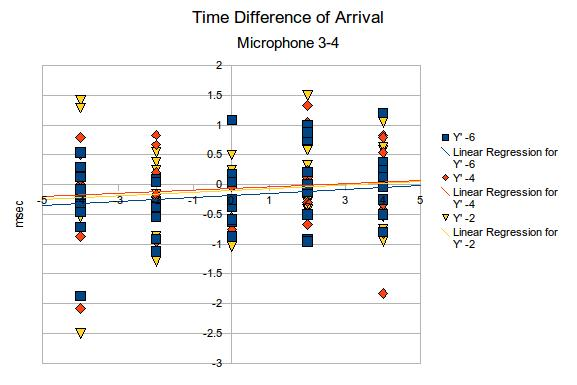
\includegraphics[scale=.55,keepaspectratio=true]{images/2_fan_9b_tdoa_34.jpg}
    \label{fig:2_fan_9b_tdoa_34}}}
  \end{center}
  \caption[Grafik TDOA dari set data FAN\_9B (1)]{Grafik TDOA dari set data FAN\_9B (1).}
  \label{fig:2_fan_9b_tdoa_1}
  \vskip .5em
\end{figure}

\begin{figure}[htp!]
\vskip 1em
  \begin{center}
    \subfigure[TDOA 1-3]
    {\fbox{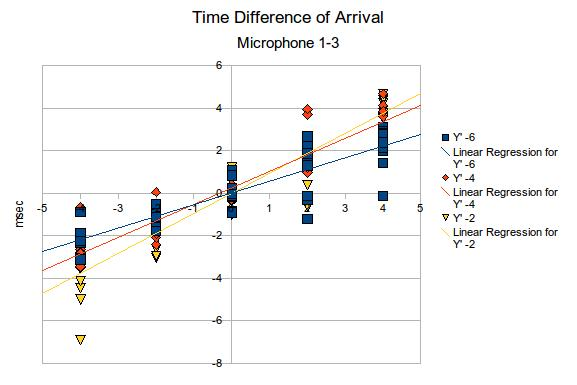
\includegraphics[scale=.55,keepaspectratio=true]{images/2_fan_9b_tdoa_13.jpg}
    \label{fig:2_fan_9b_tdoa_13}}}
    \subfigure[TDOA 1-4]
    {\fbox{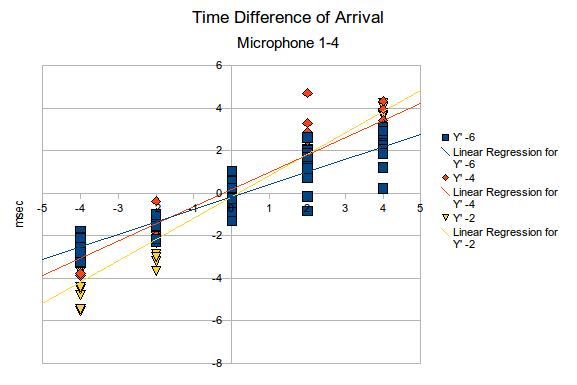
\includegraphics[scale=.55,keepaspectratio=true]{images/2_fan_9b_tdoa_14.jpg}
    \label{fig:2_fan_9b_tdoa_14}}}
  \end{center}
  \caption[Grafik TDOA dari set data FAN\_9B (2)]{Grafik TDOA dari set data FAN\_9B (2).}
  \label{fig:2_fan_9b_tdoa_2}
  \vskip .5em
\end{figure}

\begin{figure}[htp!]
\vskip 1em
  \begin{center}
    \subfigure[TDOA 2-3]
    {\fbox{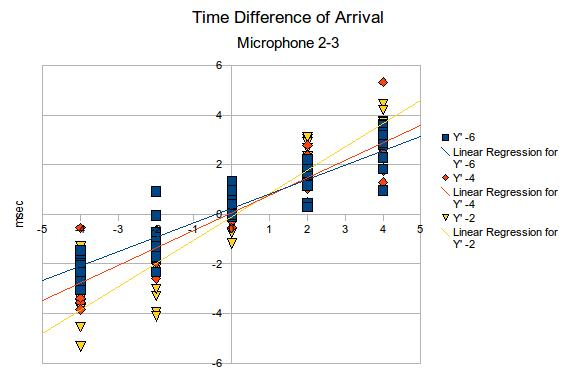
\includegraphics[scale=.55,keepaspectratio=true]{images/2_fan_9b_tdoa_23.jpg}
    \label{fig:2_fan_9b_tdoa_23}}}
    \subfigure[TDOA 2-4]
    {\fbox{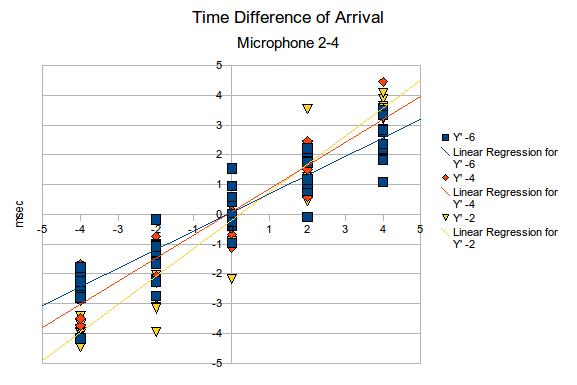
\includegraphics[scale=.55,keepaspectratio=true]{images/2_fan_9b_tdoa_24.jpg}
    \label{fig:2_fan_9b_tdoa_24}}}
  \end{center}
  \caption[Grafik TDOA dari set data FAN\_9B (3)]{Grafik TDOA dari set data FAN\_9B (3).}
  \label{fig:2_fan_9b_tdoa_3}
  \vskip .5em
\end{figure}

\begin{figure}[htp!]
\vskip 1em
  \begin{center}
    \subfigure[PtPAR 1-2]
    {\fbox{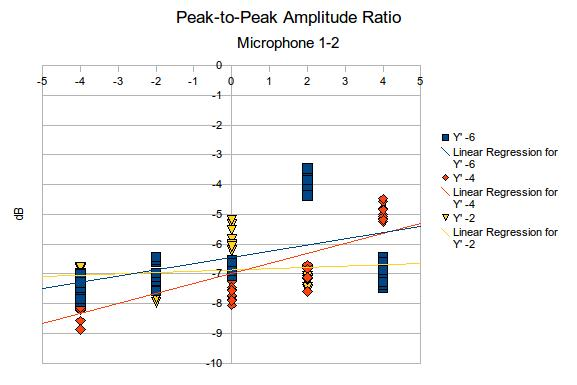
\includegraphics[scale=.55,keepaspectratio=true]{images/2_fan_9b_ptpar_12.jpg}
    \label{fig:2_fan_9b_ptpar_12}}}
    \subfigure[PtPAR 3-4]
    {\fbox{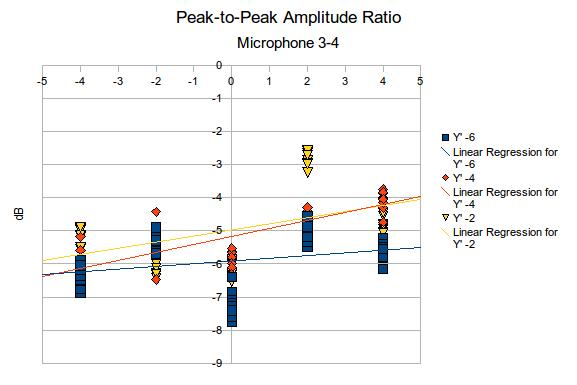
\includegraphics[scale=.55,keepaspectratio=true]{images/2_fan_9b_ptpar_34.jpg}
    \label{fig:2_fan_9b_ptpar_34}}}
  \end{center}
  \caption[Grafik PtPAR dari set data FAN\_9B (1)]{Grafik PtPAR dari set data FAN\_9B (1).}
  \label{fig:2_fan_9b_ptpar_1}
  \vskip .5em
\end{figure}

\begin{figure}[htp!]
\vskip 1em
  \begin{center}
    \subfigure[PtPAR 1-3]
    {\fbox{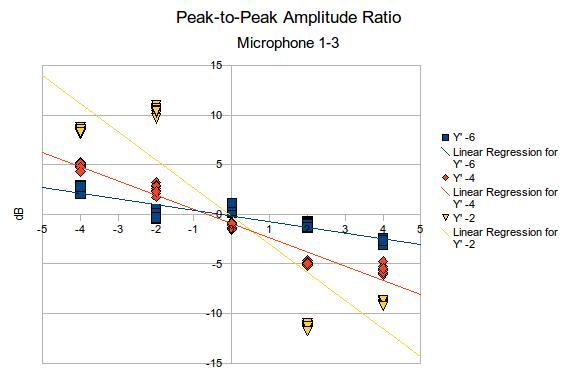
\includegraphics[scale=.55,keepaspectratio=true]{images/2_fan_9b_ptpar_13.jpg}
    \label{fig:2_fan_9b_ptpar_13}}}
    \subfigure[PtPAR 1-4]
    {\fbox{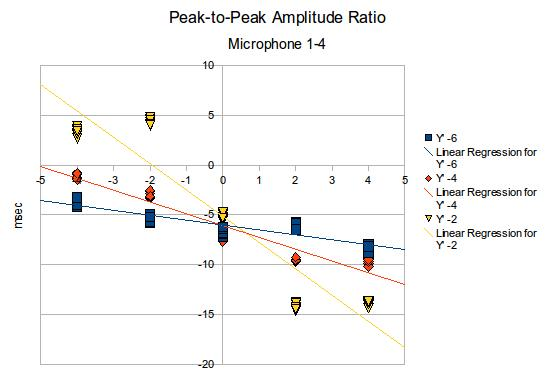
\includegraphics[scale=.55,keepaspectratio=true]{images/2_fan_9b_ptpar_14.jpg}
    \label{fig:2_fan_9b_ptpar_14}}}
  \end{center}
  \caption[Grafik PtPAR dari set data FAN\_9B (2)]{Grafik PtPAR dari set data FAN\_9B (2).}
  \label{fig:2_fan_9b_ptpar_2}
  \vskip .5em
\end{figure}

\begin{figure}[htp!]
\vskip 1em
  \begin{center}
    \subfigure[PtPAR 2-3]
    {\fbox{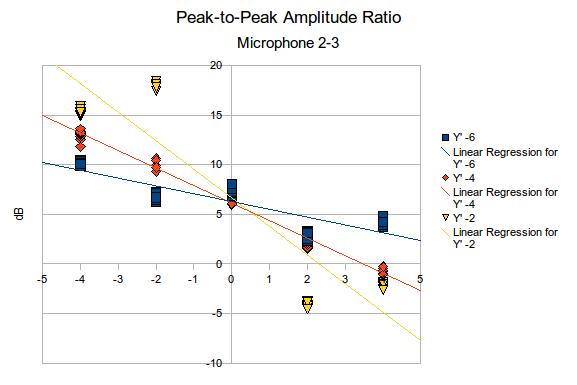
\includegraphics[scale=.55,keepaspectratio=true]{images/2_fan_9b_ptpar_23.jpg}
    \label{fig:2_fan_9b_ptpar_23}}}
    \subfigure[PtPAR 2-4]
    {\fbox{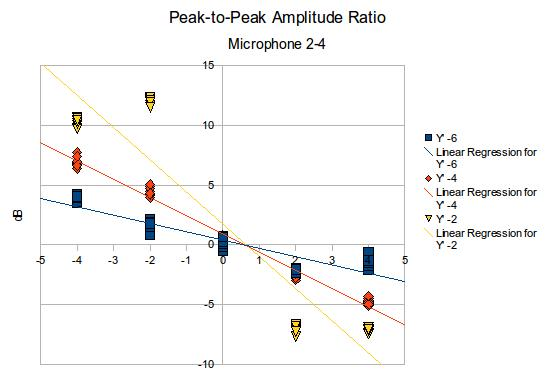
\includegraphics[scale=.55,keepaspectratio=true]{images/2_fan_9b_ptpar_24.jpg}
    \label{fig:2_fan_9b_ptpar_24}}}
  \end{center}
  \caption[Grafik PtPAR dari set data FAN\_9B (3)]{Grafik PtPAR dari set data FAN\_9B (3).}
  \label{fig:2_fan_9b_ptpar_3}
  \vskip .5em
\end{figure}

\begin{figure}[htp!]
\vskip 1em
  \begin{center}
    \subfigure[PtPAR 1-3]
    {\fbox{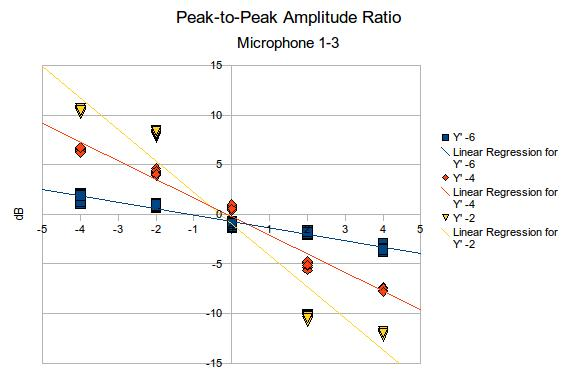
\includegraphics[scale=.55,keepaspectratio=true]{images/2_faw_7b_ptpar_13.jpg}
    \label{fig:2_faw_7b_ptpar_13}}}
    \subfigure[PtPAR 1-4]
    {\fbox{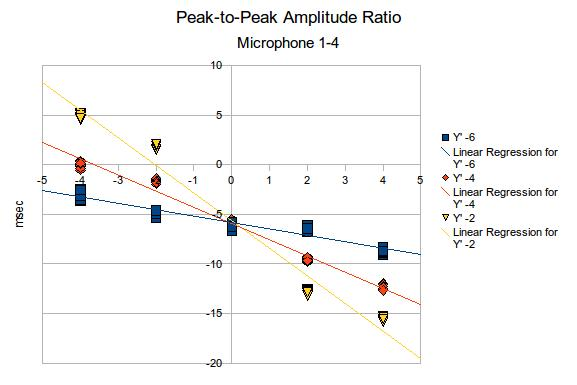
\includegraphics[scale=.55,keepaspectratio=true]{images/2_faw_7b_ptpar_14.jpg}
    \label{fig:2_faw_7b_ptpar_14}}}
  \end{center}
  \caption[Grafik PtPAR dari set data FAW\_7B (1)]{Grafik PtPAR dari set data FAW\_7B (1).}
  \label{fig:2_faw_7b_ptpar_1}
  \vskip .5em
\end{figure}

\begin{figure}[htp!]
\vskip 1em
  \begin{center}
    \subfigure[PtPAR 2-3]
    {\fbox{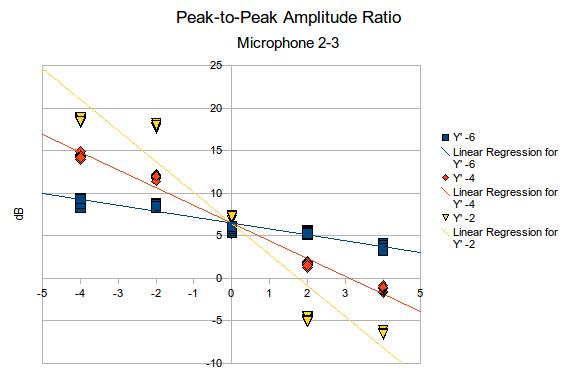
\includegraphics[scale=.55,keepaspectratio=true]{images/2_faw_7b_ptpar_23.jpg}
    \label{fig:2_faw_7b_ptpar_23}}}
    \subfigure[PtPAR 2-4]
    {\fbox{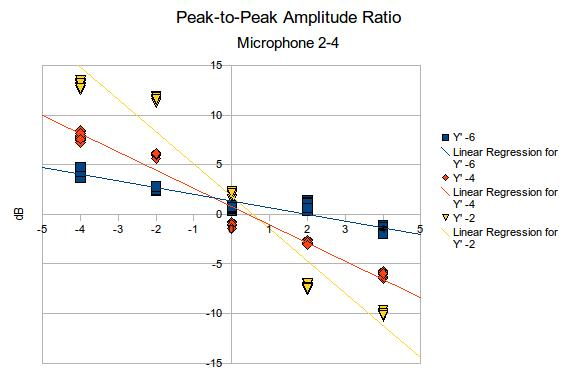
\includegraphics[scale=.55,keepaspectratio=true]{images/2_faw_7b_ptpar_24.jpg}
    \label{fig:2_faw_7b_ptpar_24}}}
  \end{center}
  \caption[Grafik PtPAR dari set data FAW\_7B (2)]{Grafik PtPAR dari set data FAW\_7B (2).}
  \label{fig:2_faw_7b_ptpar_2}
  \vskip .5em
\end{figure}



\addtocontents{toc}{\vspace{1em} \hfill {Halaman} \par}
\subsection{Pelatihan dan Pengujian Jaringan Syaraf Tiruan}

JST dilatih dengan menggunakan set data yang diperoleh pada Iterasi II. Data latih dan data uji yang digunakan berasal dari set data FAN\_9B dan FAW\_7B yang memiliki 240 data latih dan 60 data uji. Selain melakukan pelatihan dengan parameter yang sama secara berulang, parameter jumlah neuron tersembunyi dan \textit{mean squared error} (MSE) pelatihan (\textit{desired error}) juga diubah-ubah untuk memperoleh MSE pelatihan dan pengujian yang baik. Data dari proses pelatihan JST ditampilkan pada \autoref{tbl:data_pelatihan}.

JST yang diperoleh kemudian diuji dengan set data MAF\_25A dan MSD\_5B yang masing-masing memuat 50 data, serta FAN\_9B\_2 yang memuat 150 data. Data dari proses pengujian JST ditampilkan pada \autoref{tbl:data_pengujian}. Data pengujian tersebut menunjukkan bahwa MSE rata-rata terendah diperoleh dari penggunaan JST yang dihasilkan pada pelatihan ke-7. JST inilah yang nantinya akan digunakan untuk memperkirakan posisi pengguna setelah subsistem diintegrasikan ke dalam RESTU.

\begin{table}[ht!]
  \vskip 1em
\centering
\caption{Data pelatihan JST.}
\label{tbl:data_pelatihan}
\begin{tabular}{| c | c | c | c | c |}
\hline
\textbf{Pelatihan} & \textbf{Jumlah} & \textbf{Jumlah neuron} & \textbf{MSE} & \textbf{MSE} \\
\textbf{ke-} & \textbf{layer} & \textbf{tersembunyi} & \textbf{pelatihan} & \textbf{pengujian} \\
\hline
1 & 3 & 64 & 0,0009989900 & 0,010317 \\
\hline
2 & 3 & 32 & 0,0009997976 & 0,004737 \\
\hline
3 & 3 & 16 & 0,0009985201 & 0,000379 \\
\hline
4 & 3 & 16 & 0,0007484510 & 0,002396 \\
\hline
5 & 3 & 16 & 0,0004987848 & 0,004765 \\
\hline
6 & 3 & 16 & 0,0002499711 & 0,008815 \\
\hline
7 & 3 & 16 & 0,0001499649 & 0,005309 \\
\hline
8 & 3 & 16 & 0,0000999883 & 0,027223 \\
\hline
\end{tabular}
  \vskip .5em
\end{table}


\begin{table}[ht!]
  \vskip 1em
\centering
\caption{Data pengujian JST.}
\label{tbl:data_pengujian}
\begin{tabular}{| c | c | c | c | c |}
\hline
\textbf{JST Hasil} & \textbf{MSE} & \textbf{MSE} & \textbf{MSE} & \textbf{MSE} \\
\textbf{Pelatihan ke-} & \textbf{MAF\_25A} & \textbf{MSD\_5B} & \textbf{FAN\_9B\_2} & \textbf{Rata-rata} \\
\hline
1 & 0,174747 & 0,366794 & 0,309057 & 0,283533 \\
\hline
2 & 0,191638 & 0,400196 & 0,467885 & 0,353240 \\
\hline
3 & 0,201244 & 0,372975 & 0,426066 & 0,333428 \\
\hline
4 & 0,199302 & 0,219985 & 0,417764 & 0,279017 \\
\hline
5 & 0,176784 & 0,230723 & 0,445191 & 0,284233 \\
\hline
6 & 0,172334 & 0,368824 & 0,437893 & 0,326350 \\
\hline
7 & 0,139543 & 0,210295 & 0,464500 & 0,271446 \\
\hline
8 & 0,181249 & 0,356440 & 0,602393 & 0,380027 \\
\hline
\end{tabular}
  \vskip .5em
\end{table}


%%%%%%%%%%%%%%%%%%%%%%%%%%%%%%%%%%%%%%%%%%%%%%%%%%%

\subsection{Analisis Hasil}

Dari proses perancangan yang telah dilakukan, beberapa pencapaian yang telah diperoleh antara lain sebagai berikut.

\begin{enumerate}
\item Menangkap suara pengguna dengan menggunakan \textit{microphone array}, yang terdiri dari empat mikrofon, secara bersamaan memanfaatkan pustaka Portaudio. Representasi sinyal yang ditangkap disimpan dalam file yang berekstensi \texttt{raw}.
\item Menghitung TDOA dari sinyal suara yang ditangkap oleh \textit{microphone array} menggunakan metode CCC. Implementasi CCC menggunakan DFT memanfaatkan pustaka FFTW3. Implementasi telah diverifikasi kebenarannya dengan cara membandingkan hasil perhitungan yang diperoleh dari implementasi dengan hasil perhitungan yang diperoleh dari fungsi \texttt{xcorr} pada program Octave.
\item Menghitung PtPAR dari sinyal suara yang ditangkap oleh \textit{microphone array}. Implementasi telah diverifikasi kebenarannya dengan cara membandingkan hasil perhitungan yang diperoleh dari implementasi dengan hasil pengamatan grafik sinyal yang ditampilkan program Audacity.
\item Menyimpan data TDOA, PtPAR, dan posisi untuk membuat data latih dan data uji JST.
\item Melatih JST dengan nilai TDOA dan/atau PtPAR yang didapatkan selama pengambilan data latih dengan memanfaatkan pustaka FANN.
\item Menguji JST dengan nilai TDOA dan/atau PtPAR yang didapatkan selama pengambilan data uji dengan memanfaatkan pustaka FANN.
\end{enumerate}

Pada awal penelitian, parameter TDOA dan PtPAR diperkirakan dapat digunakan untuk melakukan penentuan posisi sumber suara, atau dalam hal ini adalah posisi pengguna. Parameter PtPAR terbukti dapat digunakan untuk memperkirakan posisi pengguna, sedangkan parameter TDOA tidak dapat. Meskipun demikian, parameter TDOA sebenarnya merupakan parameter yang banyak digunakan dalam penentuan posisi sumber suara sehingga tingkat keakuratannya seharusnya cukup baik. Oleh karena itu, tidak dapat digunakannya parameter tersebut dalam penelitian ini disebabkan oleh desain dan implementasi yang kurang sesuai dengan batasan masalah TDOA.

Faktor utama yang menyebabkan hasil perhitungan TDOA sangat tidak konsisten adalah faktor perangkat keras yang digunakan. Penggunaan \textit{USB sound card} yang kemudian datanya dikelola oleh program yang memanfaatkan pustaka Portaudio tidak dapat menghasilkan representasi data sinyal yang baik karena batasan waktu tidak ditepati dengan baik. Dari pengamatan, proses perekaman yang dilakukan oleh empat \textit{sound card} tidak berjalan secara bersamaan. Pengamatan dilakukan dengan memberikan penanda waktu (\textit{timestamp}) saat proses merekam mulai dan berakhir. Dari penanda waktu tersebut diketahui bahwa durasi perekaman tidak pernah terpenuhi dan durasi \textit{sound card} yang satu dengan yang lain dalam mengambil data tidak sama , meskipun semua \textit{sound card} diset untuk merekam dalam durasi yang sama. Sebagai contoh, apabila semua \textit{sound card} diset untuk merekam selama 1 detik, penanda waktu menunjukkan bahwa \textit{sound card} merekam dalam durasi $1 + \delta t$, dengan $\delta t$ bervariasi antara satu \textit{sound card} dengan \textit{sound card} yang lain. Apabila  $\delta t$ dari satu proses perekaman ke proses yang lain sama (konsisten), permasalahan mungkin dapat dipecahkan dengan memberikan \textit{offset} pada data. Dari pengamatan $\delta t$ dari satu proses perekaman ke proses yang lain tidak konsisten. meskipun nilai $\delta t$ hanya dalam orde milidetik, pada dasarnya file representasi sinyal suara yang diperoleh tidak dapat digunakan untuk menghitung TDOA. Apabila sinyal tersebut digunakan untuk menghitung TDOA, hasil perhitungan merupakan nilai yang tidak valid karena nilai tersebut sangat dipengaruhi oleh $\delta t$ sehingga tidak merepresentasikan perbedaan waktu yang dibutuhkan propagasi sinyal dari sumber suara ke mikrofon dengan baik.

Untuk memecahkan permasalahan tersebut dibutuhkan perangkat akuisisi sinyal yang mampu berjalan secara \textit{real-time}, seperti yang digunakan pada \cite{lee2005}, \cite{nakano2010}, dan \cite{park2009}. Pada prinsipnya, apabila \textit{time-constraint} yang diberikan dapat ditepati dengan baik, dengan asumsi model \textit{free-field} ideal, representasi sinyal akan memenuhi \autoref{eq:sinyal_ditangkap}.
